\documentclass{apa}

\usepackage[utf8]{inputenc}
\usepackage[american]{babel}

\usepackage{epsfig}
\usepackage{apacite}
\usepackage{graphicx}
\usepackage{epsfig}
\usepackage{amsmath}
\usepackage{url}
\usepackage{bm}

% ---------- watermark -----------
\usepackage[firstpage]{draftwatermark}
\SetWatermarkAngle{0}
\SetWatermarkFontSize{0.25cm}
\SetWatermarkVerCenter{1.15cm}
\SetWatermarkLightness{0.5}
\SetWatermarkHorCenter{14cm}
\SetWatermarkText{\shortstack[l]{
Navarro, D. J. and Perfors, A. (2011). Hypothesis generation, the positive \\
test strategy, and sparse categories. Psychological Review, 118, 120-34 \\
http://dx.doi.org/10.1037/a0021110
}}
\SetWatermarkScale{1}
% -------------------------------


\newcommand{\given}{\, | \,}
\newcommand{\oracle}{{\mathcal{O}}}
\newcommand{\uses}{=}
\newcommand{\rulesize}{n}
\newcommand{\h}[1]{\textsc{#1}}
\newcommand{\ruleset}{\mathcal{H}}
\newcommand{\queryset}{\mathbf{X}}
\newcommand{\universe}{\mathbf{\Omega}}

\newcommand{\p}{P}

\title{Hypothesis generation, sparse categories and the positive test strategy}


\twoauthors{\normalsize Danielle J. Navarro}{\normalsize Andrew Perfors}
\twoaffiliations{School of Psychology \\ University of Adelaide}{School of Psychology \\ University of Adelaide}
\rightheader{Generating and testing sparse hypotheses}
\shorttitle{Generating and testing sparse hypotheses}
\leftheader{Generating and testing sparse hypotheses}

\abstract{We consider the situation in which a reasoner must induce the rule that explains an observed set of data but the hypothesis space of possible rules is not explicitly enumerated or identified. The first part of the paper demonstrates that as long as hypotheses are sparse (i.e., index less than half of the possible entities in the domain) then a positive test strategy is near-optimal. The second part of this paper then demonstrates that a preference for sparse hypotheses (a sparsity bias) emerges as a natural consequence of the family resemblance principle; that is, it arises from the requirement that good rules index entities that are more similar to one another than they are to entities that do not satisfy the rule.}

\begin{document}
\maketitle

\section{Introduction}

Uncovering the rules that govern the observations that we make is a fundamental inductive inference problem, covering many substantively different domains and several formally distinct learning problems. In its most general form, the learner must induce the rule on the basis of a collection of observations and some information as to which observations satisfy the rule. Across domains, this broad problem includes children acquiring grammatical rules \cite<e.g.,>{chomsky57}, scientists searching for physical laws \cite<e.g.,>{popper35,kuhn70}, people learning rule-governed concepts \cite<e.g.,>{brunergoodnowaustin56} and many others. In this paper we consider the problem of active learning, in which it is the learners responsibility to make queries regarding the phenomenon of interest in order to uncover the true rule that describes it. This learning problem has two distinct parts: the {\it hypothesis generation problem}, in which plausible candidate rules must be proposed, and the {\it hypothesis testing problem}, in which appropriate tests of those hypotheses must be constructed.

%Variations on the problem turn up in the acquisition of linguistic knowledge \cite<e.g.,>{chomsky57}, the construction of scientific theories \cite<e.g.,>{popper35,kuhn70}, and the learning of novel concepts \cite<e.g.,>{brunergoodnowaustin56,Ashby1988,Nosofsky1994a,Rouder2004}, and in a range of other contexts. In its most general form, the learner has made a collection of observations and received some information as to which observations satisfy the rule. One particular case of interest is the ``active learning'' problem, in which the learner chooses which observations to make. Experimental design in science is a good example of this sort of problem, as is XXXXXX.


The hypothesis testing problem is well-studied in the literature on reasoning and decision-making, and displays a striking empirical regularity. In general, people prefer to employ a {\it positive test strategy}, or PTS \cite<see>[for an overview]{nickerson98,mckenzie05}. The PTS can be characterized as the tendency to ask questions that will yield an affirmative response if the hypothesis currently under consideration is true \cite{klaymanha87}. Although it is sometimes difficult to disentangle from the matching bias (\citeNP{evans1972,evanslynch73,Evans1998}, see also \citeNP{yama2001}), the PTS is pervasive. It is observed in
rule-learning problems \cite<e.g,>{wason60,taplin75,tweneyetal80,klaymanha89}, the four-card selection task \cite<e.g.,>{wason68,Jones2001}, scientific research \cite<e.g.,>{mahoneydemonbreun77,mynattetal78,dunbar93}, and many other contexts \cite{nickerson98}. The bias to use a PTS can be ameliorated in some situations \cite<e.g.,>{Johnsonlaird1972,Cheng1985,cosmides89}, but is rarely completely eliminated. Moreover, although there are some senses in which it represents a logical error \cite{wason60,platt64,wason68,johnsonlairdwason70}, the PTS can be a highly effective learning strategy when certain assumptions are met \cite{klaymanha87,klaymanha89,oaksfordchater94,austerweilgriffiths08}.

Hypothesis generation is less well-studied by comparison, but is presumably tied to the question of what kinds of rules people find to be {\it a priori} more plausible than others. Within the rule-based categorization literature, for instance, it is typical to assume the existence of a relevant class of possible rules \cite{Nosofsky1994a,Ashby1988,goodmanetal08,Erickson1998}, and there has long been a recognition that learning involves strategic shifts in the learner's choice of hypothesis \cite<e.g.>{Goodnow1955,Levine1959,brown74}. There has been some exploration of the hypothesis generation problem in more general contexts than categorization \cite<see>{gettysfisher79,gettysmehlefisher86,koehler94,thomas08}, usually in isolation from the hypothesis testing problem. Those studies that have linked the generation problem to the testing problem have tended to focus on empirical questions about how people's strategies for hypothesis formation affect their overall performance \cite<e.g.,>{klahrdunbar88,farrisrevlin89,adsitlondon97}. There is relatively little work addressing the theoretical question of which hypothesis formation strategies {\em should} be followed; the closest work that we are aware of is that of \citeA{cherubinietal05}, who present empirical evidence suggesting that people incrementally form hypotheses that are informative with respect to observed data.

In this paper we present an analysis of the active learning problem that considers the hypothesis testing and hypothesis generation problems together. In the first part of the paper, we extend previous results that derive the PTS as a near-optimal learning strategy when hypotheses are {\it sparse} (that is, when they index only a minority of possible entities). In the second, more novel part of the paper, we turn to the hypothesis generation problem and show that sparsity itself is a consequence of the more basic requirement that rules correspond to ``good'' categories. We conclude by discussing some of the assumptions and simplifications incorporated into this analysis.


\section{Positive Tests for Sparse Hypotheses}

Several studies suggest that the positive test strategy can be a rational learning strategy \cite{oaksfordchater94,austerweilgriffiths08,klaymanha87} as long as one key assumption is met. All of the formal results invoke some form of ``sparsity assumption'', in which the hypothesis is consistent with only a minority of logically possible observations \cite<see>[for a discussion]{mckenzie05}. Although the psychological ideas behind these results are quite general, they are limited in two respects, both of which \citeA{klaymanha87} briefly discussed but did not include in their formal analysis.

First, the derivations all assume that the learner considers only a single hypothesis at a time.  Although there is evidence that people often do this \cite<e.g.,>{taplin75,mynattetal77,dohertyetal79}, it is not always the case. Many studies explore how entertaining multiple hypotheses affects the process of inference, with some finding that it helps \cite<e.g.,>{klahrdunbar88,klaymanha89}, some finding that it does not \cite<e.g.,>{tweneyetal80,freedman92}, and some finding that it depends \cite<e.g.,>{farrisrevlin89,mcdonald90}. In view of this, it would be useful to extend the existing formal results to cover the multiple hypothesis case.

Second, previous derivations analyze the PTS as a method for uncovering as much information as possible about the learner's hypothesis, not as a method for optimally identifying the true rule. While these are closely related goals, they are not necessarily equivalent. If the goal of the learner is to identify the true rule rather than simply to test the current hypothesis, it is important to have a formal analysis that explores the effect of different learning strategies on {\it all} of the candidates in the learner's hypothesis space -- on all of the possible rules that they could consider.

In this section we retain the critical assumption of sparsity, but extend previous results by addressing the two issues discussed above. That is, we present an analysis that accommodates multiple hypotheses, and derives the PTS in a situation where the goal is to uncover the correct rule as quickly as possible (rather than extract information about the current hypothesis). Our results suggest that the effectiveness of the PTS can change as hypotheses are eliminated and the proportion of hypotheses that are explicitly available to the learner changes.


\subsection{The ideal learner case}

The kind of active learning problems in which we are interested is best exemplified by the traditional game of ``twenty questions.'' In this game, one player (the oracle) thinks of an object, and the other player (the learner) can pose queries to the oracle. These queries must be yes-or-no questions, and the oracle must answer truthfully. Strictly speaking, the learner's goal in this game is to ask questions in such a way as to identify the object using 20 questions or fewer, but in practice the goal is to do so using as few questions as possible. An interesting variation of the game is the ``rule learning'' task introduced by \citeA{wason60}. The rule learning game differs from twenty questions in that the oracle thinks of a rule rather than an object, and constrains the allowable queries to be of the form ``does $x$ satisfy the rule?'' where $x$ is an object. For example, in one game the oracle might think of a rule about numbers, such as \h{perfect squares}. The learner's queries might include items like 7, 15, and 16, to which the oracle would reply ``no'', ``no'' and ``yes'' respectively. In the analysis below, we assume that the learning task is the Wason variant.

How would an ideal learner approach this game? Following the approach taken in the formal literature on rule-based categories \cite{Nosofsky1994a,Ashby1988,goodmanetal08,Erickson1998} we assume that the learner has a set of (not necessarily explicit) plausible hypotheses $\ruleset$ about the rule. This is the learner's hypothesis space. (We defer questions about the origin of $\ruleset$ to the next section.) Let $h$ be a specific hypothesis about a rule, $x$ be one possible query item, and $\mathcal{X}$ be the set of all possible queries that the learner might ask in the game. For simplicity, we suppose that the learner places an initial uniform prior over the hypotheses (so that $\p(h) = 1/N$, where $N$ is the current total number of hypotheses in $\mathcal{H}$).  If the learner poses query $x$ and the oracle gives response $r$, Bayes' theorem tells us that the degree of belief associated with hypothesis $h$ is given by:
%%
\begin{equation}
\p(h \given r,x) = \frac{\p(r \given h,x) \p(h)}{\sum_{h^\prime} \p(r \given h^\prime,x) \p(h^\prime)}.\label{likelihood}
\end{equation}
%%
The term $\p(r \given h,x)$ denotes the probability that the oracle would have given response $r$ to query $x$ if hypothesis $h$ were true. This probability is 1 if the query item is contained in the rule corresponding to the hypothesis and 0 if it is not.  Thus, all hypotheses that are inconsistent with the oracle's answer are eliminated and all others are retained.  If we let $n_c$ denote the number of hypotheses that are consistent with the set of responses and queries so far, then the degree of belief associated with hypothesis $h$ is now given by:
%%
\begin{equation}
\p(h \given r, x) = \left\{ \begin{array}{cl} \frac{1}{n_c} & \mbox{ if $h$ is consistent with all responses} \\ 0 & \mbox{ otherwise} \end{array} \right. .
\end{equation}
%%
\noindent
Because any hypothesis that is not consistent with the responses so far is eliminated, at every stage in the game the learner has a collection of not-yet-falsified hypotheses, each of which is equally plausible. Though simple, this setup closely mirrors the framework used by \citeA{popper35}, in which a single disconfirming observation is sufficient to falsify a hypothesis, but many confirming observations are needed to provide strong evidence in favor of the hypothesis. It is consistent with the classic ``win-stay/lose-shift'' strategy pervasive in human learning \cite{Goodnow1955,Levine1959,brown74}, in which people retain a hypothesis as long as it makes correct predictions, but discard it the moment it makes an incorrect one.

The learner's goal is to choose a query $x$ in such a way as to allow the true rule to be identified as quickly as possible.  The learner knows that the oracle is either going to say ``yes'', in which case there will be some number of hypotheses $n_y$ remaining, or the oracle is going to say ``no'', in which case there will be $n_n = N - n_y$ hypotheses remaining. For instance, one query might be consistent with only 1\% of possible rules, while another one could be consistent with 50\% of the rules. For the first query, there is a 1\% chance that the oracle will eliminate 99\% of the possible rules and a 99\% chance that it will eliminate 1\% of the rules; for the second, 50\% of the rules will end up eliminated regardless of what the oracle says.

From an information theoretic perspective \cite<e.g.,>{mackay03} it is not difficult to show that the second type of query is superior. If the aim is to identify the rule as quickly as possible, a rational learner should choose the item $x$ that is expected to minimize the posterior entropy $H(h \given x, r)$ of her belief about the identity of the correct rule, since this corresponds to a state of maximal knowledge and minimal uncertainty.\footnote{There are, of course, other ways that the learner's goal could be formalized \cite<see, e.g.,>[for a discussion]{nelson05}, including minimizing the number of queries or maximizing the diagnosticity of the next question. We chose this because it is a reasonable goal, and because it is consistent with empirical findings about how human learners appear to gather information \cite{nelsonetal01}.}  The learner should therefore pick the $x$ that is expected to return the most information about the true rule. Formally, the expected entropy is given by:
%%
\begin{eqnarray}
E_r[H(h \given x, r)]
&=& \frac{n_y \ln n_y + n_n \ln n_n}{N}, \label{ent2}
\end{eqnarray}
%%
\noindent
where $n_y + n_n = N$. The important thing to note is that this function, which is explicitly derived in the Appendix and illustrated for $N=32$ in Figure~\ref{entropy}a, is minimized when $n_y =n_n = N/2$. Thus, the optimal query $x$ is one that is true for exactly half of the not-yet-eliminated hypotheses. This corresponds to the ``bisection'' search method that people intuitively prefer to use in simpler situations. Games in which the learner needs to identify an unknown person often start with queries about gender for exactly this reason.

\begin{figure}
\begin{center}
\begin{tabular}{cc}
\epsfig{file=deterministicrules.eps,width=7cm} &
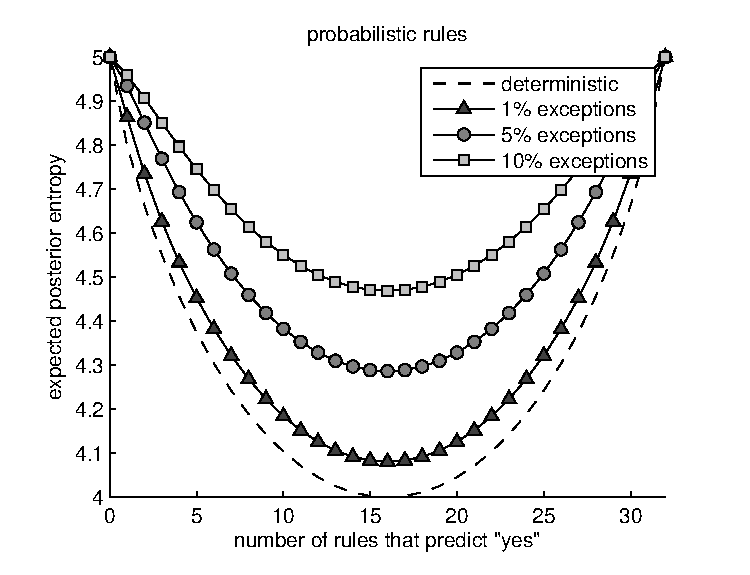
\epsfig{file=probabilisticrules.eps,width=7cm} \\
(a) & (b)
\end{tabular}
\caption{Expected posterior entropy (in bits) as a function of $n_y$, for a domain with $N=32$ objects. Panel a shows the result for deterministic rules (Equation~\protect\ref{ent2}), whereas panel b shows what happens when some proportion of the items $\phi$ are allowed to constitute exceptions to the rules. The qualitative pattern is the same in all cases, regardless of whether the rules are deterministic or probabilistic.}
\label{entropy}
\end{center}
\end{figure}

\subsection{Extension to probabilistic rules}


The formalism for active learning described earlier assumes that rules are deterministic, allowing no exceptions, and that the oracle gives perfect feedback. This is of course a simplification, given that many (perhaps most) rules allow exceptions. We can capture this by supposing that the proportion of exception items is $\phi$ (or, equivalently, that the oracle makes mistakes for a proportion $\phi$ of the items). When this occurs, no rule is ever perfectly falsified, since any disagreements between the rule and the oracle's answer might have been errors by the oracle or genuine exceptions to the rule. Under such circumstances, the calculation of the expected posterior entropy is somewhat more complicated: a derivation appropriate to this case is provided in the Appendix. The important point, however, is that the qualitatively important features of the expected entropy function are unchanged. This is illustrated in Figure~\ref{entropy}b, which plots the expected posterior entropy as a function of $n_y$ for several different levels of $\phi$. The key point is that the curves are all still U-shaped, with a minimum value at $n_y = N/2$. Since these characteristics are the ones that our analysis relies upon, it is clear that our results generalize to probabilistic rules.

%Since it is only these features that we rely upon in our subsequent discussion of the PTS for the deterministic case, it is clear that the discussion generalizes to probabilistic rules.


\subsection{The partial-information case}

The previous analysis relies on the assumption that the learner has access to $\mathcal{H}$, the full set of plausible hypotheses, and is able to choose $x$ in such a way as to ensure that $n_y=n_n$. Under these assumptions, there ought not to be any PTS bias. However, these assumptions are not satisfied in the Wason (1960) task or the twenty questions game more generally. In most cases, the learner has only very limited information to work with: for instance, it is typically assumed that the learner can only keep a small number of hypotheses in working memory, perhaps only one hypothesis \cite<see>{dougherty03}. If so, it is likely that only this limited subset of explicit hypotheses $\mathcal{H}_E$ can be used to guide the choice of $x$. For the current purposes, we assume that $\ruleset_E$ is a more-or-less random subset of $\ruleset$ \cite<e.g.>{Nahinsky1970,Williams1971}. As long as $\ruleset$ only contains ``plausible hypotheses'' this assumption seems reasonable: it amounts to the assumption that people ignore ``implausible'' hypotheses, and choose randomly among the ``plausible'' ones. As such it is broadly consistent with models of hypothesis generation \cite{gettysfisher79,thomas08} which assume that people form hypotheses in a sensible fashion.

To formalize the hypothesis testing problem when the learner has access only to the explicit subset $\ruleset_E$, note that the set of $N$ rules and $M$ entities produces an $N \times M$ binary ``truth matrix'', whose $ij$th element is 1 if the $i$th hypothesis in $\mathcal{H}$ predicts an affirmative response to the $j$th possible query, and 0 if it does not. In the simplest case, this is an unstructured matrix in which the cells are independent of one another. We let $\theta$ denote the probability that any element takes on value 1. In this situation, if the learner chooses $x$ completely at random, then the number of hypotheses that predict an affirmative response to any given query will be binomially distributed:
%%
\begin{equation}
n_y \sim \mbox{Binomial}(\theta,N).
\end{equation}
%%
If it happens to be the case that $\theta=1/2$, then the expected number of hypotheses that would yield an affirmative response $n_y$ is $N/2$; in other words, the query has a reasonable chance of being optimal with respect to $\mathcal{H}$. However, for other values of $\theta$ this is not the case. In particular, if the hypothesis space is {\it sparse}, then $\theta < 1/2$, meaning that most hypotheses would yield an affirmative response only to a minority of possible queries.  In this situation most queries will be suboptimal, since $n_y$ will probably be smaller than $n_n$. If the learner has no hypotheses in mind (i.e., $\mathcal{H}_E$ is empty) then there is nothing the learner can do to improve matters.  But if she has a small number of hypotheses $\mathcal{H}_E$ in mind, then choosing queries to which those hypotheses yield affirmative responses will boost $n_y$, and thus improve the efficiency of the query.  This is true even if the learner does not know the sparsity, and even if the explicit hypotheses $\mathcal{H}_E$ themselves are not sparse, as long as the average sparsity $\theta$ of the hypotheses in the entire space is less than 1/2; the entropy is related to how efficiently the query eliminates hypotheses across the entire hypothesis space.

\subsection{Summary}

The basic result states that as long as the hypotheses tend to be sparse and the learner does not have access to all relevant hypotheses at all times, it is sensible to adopt the PTS with respect to the set of hypotheses that the learner {\it does} have access to. This is true whether the rules are probabilistic or deterministic. This occurs because a sparse hypothesis space means the oracle is expected to produce too many ``no'' responses with respect to $\mathcal{H}$, and a strategy that is highly biased towards a ``yes'' response with respect to  $\mathcal{H}_E$ is the best way to overcome it.  This does not mean that such a strategy will {\it necessarily} or {\it entirely} counteract such a bias -- it depends on the strength of the bias and the details of the specific rules and hypothesis space. It does mean that, in general, the PTS will counteract it better than most other strategies would. This is because, even if some rules are not currently available to the learner, the oracle's response will still be informative about them (ruling out those that are inconsistent from ever being considered).

An interesting corollary of this result is the implication that as the number of implicit hypotheses decreases or the sparsity of the remaining hypotheses increases the extent of the bias should reduce. When all remaining hypotheses are explicit the bisection strategy will become optimal. In fact, empirical findings do suggest that beginning with a confirmatory strategy and moving toward a disconfirmatory one is more effective \cite{mynattetal78}. Our analysis can help to explain other experimental results as well.  For instance, the notion that the PTS may emerge because of a capacity limitation is consistent with empirical evidence that increasing the number of alternative hypotheses considered in $\ruleset_E$ may improve learning \cite{klaymanha89}.



\section{Hypothesis Generation, Sparse Categories and Family Resemblances}

The main assumption made by all rational analyses of the PTS is that hypotheses are sparse. Regardless of the precise set up, some assumption of this form appears to be necessary. In light of this, it is natural to ask what theoretical justification exists to support this assumption. While there are some situations in which hypotheses are necessarily sparse \cite{austerweilgriffiths08}, most analyses have relied on the fact that the sparsity assumption appears to be {\it empirically} justified  \cite{klaymanha87,oaksfordchater94}. While this is reassuring, it is somewhat unsatisfying at a theoretical level: a theoretical account of the PTS that makes use of the sparsity assumption should, ideally, be accompanied by a theoretical explanation of sparsity itself. In this section, we seek to provide this theoretical basis for sparsity. We begin by discussing the evidence for the sparsity assumption, and go on to derive sparsity from more basic premises.

\subsection{The empirical evidence for sparsity}

Regardless of what the correct theoretical explanation for the phenomenon is, there is considerable empirical evidence that people do have sparse hypothesis spaces. Most obviously, people's hypotheses about rules are presumably heavily reliant on natural categories. For instance, in Wason's number game, the learner might propose a sparse rule such as ``multiples of two'' because he or she is relying on the natural category of ``even numbers''. Therefore if natural categories are sparse, one would expect that the hypotheses that people form in the context of an active learning problem would also be sparse. It is intuitively obvious that natural categories are indeed sparse: only a minority of entities in the world belong to the category ``dog'', for instance. Even when we consider the more realistic situation where the domain is somewhat restricted, sparsity is still the norm. That is, even if we restrict ourselves to a discussion of animals (rather than all entities in the world) it is still the case that most animals are not dogs. Not surprisingly, therefore, experiments aimed at eliciting information about the structure of natural categories support the intuition that natural categories are sparse (e.g., \citeNP{DeDeyne2008}).

Even in the more specific context of hypothesis generation -- as opposed to category learning generally -- there is empirical evidence for sparsity. In previous work \cite{perforsnavarro09} we found that the number rules people spontaneously construct are extremely sparse.  Similarly, in a more complex study in an automotive context \cite{mehle82}, participants  appeared to prefer sparse theories; indeed, the more they knew about the domain, the sparser their hypotheses tended to be. In short, hypothesis sparsity is an empirical regularity regarding human hypothesis generation.


\subsection{Sparsity is not a logical necessity}

Just as it is obvious that natural categories are sparse, it is also obvious that this sparsity is not a logical necessity. If the domain in question consists of a set of $M$ objects, then we can associate every possible rule $h$ with the category of objects that satisfy the rule. In total, there are $2^M$ distinct categories that are possible in this domain, any of which might correspond to the category in question. Clearly, if the learner treats each of these categories as equally plausible, then no sparsity bias will emerge: for every category containing $K$ entities, there exists a complementary category containing $M-K$ entities. As a consequence, the average sparsity of will be exactly $1/2$. While this is hardly a novel insight, it illustrates a simple but important point: sparsity requires a {\it psychological} explanation.

A natural place to look for such an explanation is to examine how sparsity is captured within formal models of human categorization \cite<e.g.,>{Nosofsky1984,Anderson1991,Kruschke1992,Love2004,griffithssanborncanininavarro08}. Most of these models do possess a sparsity bias, and in the majority of cases this bias is imposed because the model assumes that categories form a {\it partition} of the stimuli. That is, the models assume that individual entities are assigned to exactly one category, and as a consequence it is almost impossible for the models to produce non-sparse category assignments. This is illustrated in Figure~\ref{sparsereps}a, in which a partition of six objects has one category of size 3 {\tt(A,B,C)}, one of size 2 {\tt(D,F)} and one of size 3 {\tt(E)}, corresponding to a very sparse representation. The key point here is that theoretical models tend to impose sparsity via the structure of the category representation, which in this instance is a partition.

Of course, it is not true in general that categories are organized into partitions. In fact, there is considerable evidence that natural concepts can be organized into a range of different structures: besides partitions, human mental representations can take the form of hierarchies, spaces, networks, grammars and many other possibilities \cite<see>[for an overview]{kemptenenbaum08}. Even so, it does appear to be the case that  sparsity holds across these structures. To give a single example, the most common alternative to partitions are hierarchies. As illustrated in Figure~\ref{sparsereps}b, if every node in the hierarchy maps to a category, then the overall representation tends to be sparse. The only way to avoid sparsity is to exclude the ``singleton'' categories category (i.e., the terminal nodes), and then construct the most ``top-heavy'' tree possible: over 6 objects, this would produce the categories {\tt(A,B)}, {\tt(A,B,C)}, {\tt(A,B,C,D)}, {\tt(A,B,C,D,E)}, and {\tt(A,B,C,D,E,F)} which has sparsity just over $1/2$. However, this is an extremely atypical case: in general, trees tend to be sparse.

In view of this, one might be tempted to think formal models {\it necessarily} impose sparsity. However, this is not the case. For instance, in the connectionist approach to semantic representation the main commitment is to some form of ``distributed representation'' \cite{rogers04}, which may or may not be sparse. Similarly, overlapping clustering \cite{Shepard1979} produces stimulus representations in which objects can belong to any number of categories, and there are no constraints on how categories overlap. Again, these representations can be sparse, but they do not have to be. For instance, Figure~\ref{sparsereps}c shows a distributed representation over six objects produced by a set of overlapping nonsparse categories. Thus, while sparsity is common among the representational systems used in cognitive science, it is not a required feature of formal models in general. It is possible to devise representational systems that systematically violate sparsity,\footnote{Indeed, this is trivially easy to do. Let $F$ denote some formal system that generates category system $c$ (defined over a set of $M$ objects) with probability $p$, and produces an expected sparsity of $\theta$. Then, we may define $F^*$ to be the formal system that generates the ``complementary'' category system $c^*$ with probability $p$. By complementary we mean that if the $k$-th category in $c$ indexes the set of $q$ items $c_{k1},\ldots,c_{kq}$, then the $k$-th category of $c^*$ indexes the other $M-q$ items in the domain (as an example, the category systems shown in Figures~\ref{sparsereps}a and \ref{sparsereps}c are complementary). The expected sparsity of representations produced by formal system $F^*$ will necessarily be $1-\theta$. Thus, if $F$ is sparse, then $F^*$ is not. In exactly the same way that categories are not logically constrained to be sparse, neither are formal systems for organizing categories. As before, one might argue that the complementary system $F^*$ to a sensible sparse system $F$ tends to be somewhat implausible, but such an argument would rely on the very thing we are trying to explain: human preferences for sparse representations.} but since this would be inconsistent with the empirical evidence, researchers have avoided doing so.

The key thing to take from the previous discussion is this: the general tendency to see sparse formalisms for category representation is a {\it consequence} of the empirical data, not an explanation of that data. To see this, suppose that we were to argue that -- although sparsity is not a logical requirement -- it emerges because people rely on structured representations (e.g., partitions) that are sparse. This argument would be correct as far as it goes, but it begs the question as to why some (sparse) formalisms are plausible, but other (non-sparse) possibilities are not. If we try to justify the preference for sparse formalisms by reference to the empirical data (human categories are sparse) then we are right back where we started: ``explaining'' sparsity by pointing out that human categories are sparse. In short, we have {\it no} explanation at all for the sparsity of categories. A more general theoretical principle is required.



\begin{figure}
\begin{center}
\hspace*{-.5cm}\begin{tabular}{ccc}
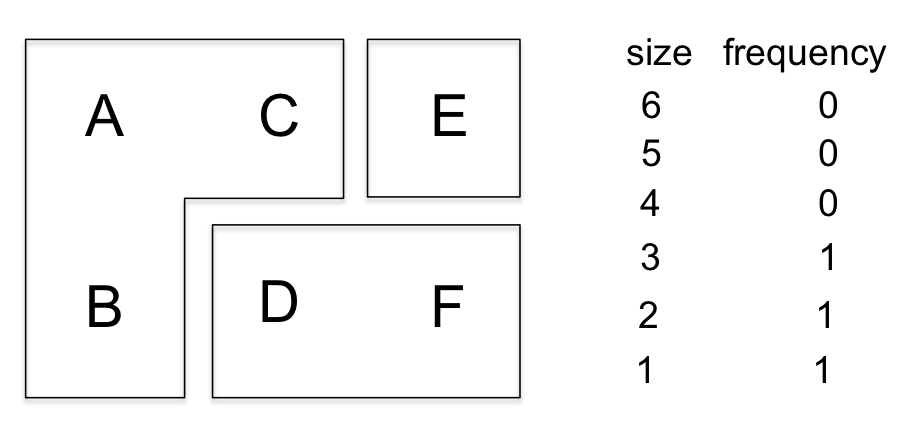
\epsfig{file=partition.eps,width=5cm} &
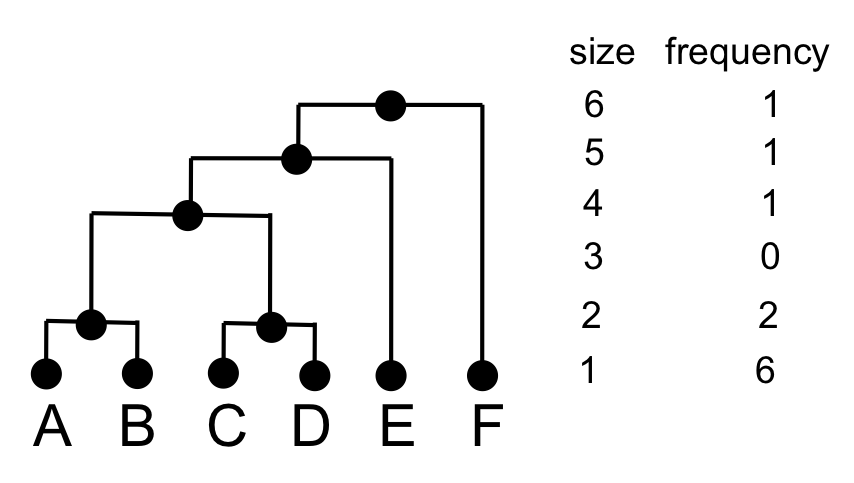
\epsfig{file=hierarchy.eps,width=4.5cm} &
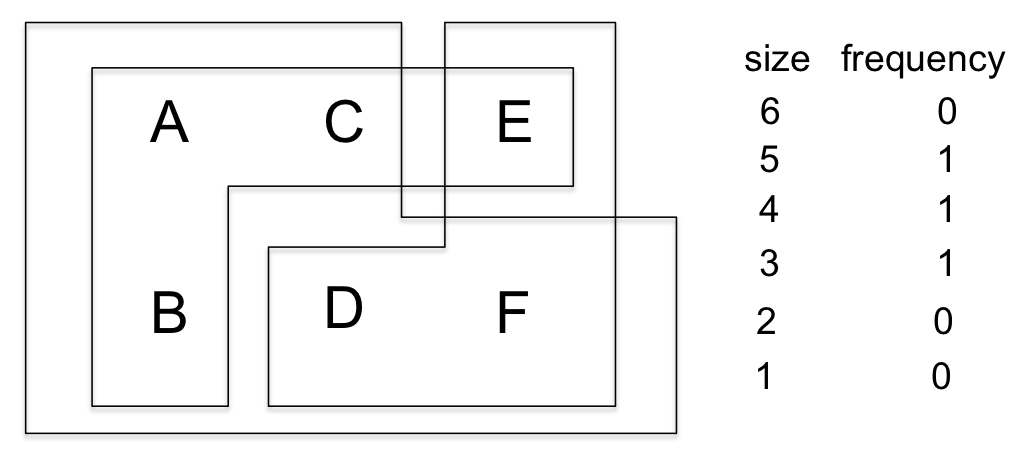
\epsfig{file=flippedpartition.eps,width=5.5cm} \\
(a) & (b) & (c)
\end{tabular}
\caption{Are formal representations sparse? Partitions (panel a) are almost always sparse, trees (panel b) are usually sparse, while distributed representations (panel c) can be sparse or non-sparse as desired.} \label{sparsereps}
\end{center}
\end{figure}






\subsection{The family resemblance principle as a potential explanation}


%The previous analysis relies on the assumption that explicit hypotheses $\ruleset_E$ are generated from the sparse hypothesis space $\ruleset$, and like many authors \cite<e.g.>{Nahinsky1970,Williams1971} we assume the sampling is largely random. As long as $\ruleset$ only admits ``plausible'' hypotheses, this does not seem unreasonable, and is consistent with those models of hypothesis generation \cite{gettysfisher79,thomas08} that assume hypotheses are generated in a sensible fashion. However, this merely begs the question: what makes one rule any ``better'' or more ``plausible'' than another? We  answer by observing that every hypothesized rule $h$ can be mapped onto a category: the set of entities that are consistent with that rule. If there are $M$ entities in the domain, then there are a total $2^M$ logically possible categories that a rule might refer to. Our assumption is that some of these categories are better than others, and that the learner's hypothesis space $\ruleset$ includes only a small number $N \ll 2^M$ of these categories. Moreover, it seems plausible that the learner will admit only those rules that correspond to categories that are ``good'' in some sense.

At this point it is clear that we are looking for a psychological principle that is (a) satisfied by natural categories, (b) consistent with existing formal models, and (c) explains the emergence of the hypothesis sparsity effect. One candidate for this principle is {\it family resemblance}. Put simply, the family resemblance principle states that a category is a good one if the members of the category tend to more similar to one another than they are to entities that do not belong to category. The fact that natural categories satisfy the family resemblance principle was pointed out by \citeA{rosch78}, and the principle is reflected in some form in most models of categorization \cite<e.g.,>{Nosofsky1984,Anderson1991,Kruschke1992,Love2004,griffithssanborncanininavarro08}. So it is clear that family resemblance meets the criteria (a) and (b) above. Additionally, variations of this principle provide much of the foundation for the statistical theory of classification \cite<see>{Gordon1999}, so there is something of a ``rational flavor'' to the idea. In short, the family resemblance principle is a central element in any psychologically plausible theory of concepts.

In the next section, we address the third criterion, and show that sparsity is a logical consequence of the family resemblance principle itself. When doing so, it is helpful to distinguish the ``pure'' idea of family resemblance from the formal models that implement this principle. As noted above, formal models often enforce sparsity by assuming that categories form a partition or a hierarchy, or some related structure that is necessarily sparse. However, these restrictions are not strictly required by the basic idea of family resemblance. The critical constraint that the family resemblance idea implies is this: a good category is one that groups together items that are more similar to one another than they are to other items. Thus the derivation that follows seeks to show that that sparsity follows from the ``group by similarity'' idea.

\subsection{On the goodness of categories}

To begin with, we need to formalize the family resemblance principle. Suppose that we have some hypothesized rule $h$ that picks out a category, and let $\bm{x}_h$ denote the set of entities that belong to that category. If we let $s(x_i, x_j)$ denote the similarity between entities $x_i$ and $x_j$, then the average ``within category'' similarity $s_{\rm in}(\bm{x}_h)$ is given by
%%
\begin{equation}
s_{\rm in}(\bm{x}_h) = \frac{1}{m_h(m_h-1)}\sum_{x_i \in \bm{x}_h}  \sum_{x_j \in \bm{x}_h} s(x_i,x_j) \label{within}
\end{equation}
%%
where $m_h$ denotes the number of entities in the category (out of a total of $M$ entities in the domain), and the summations are taken over all $i \neq j$. This is graphically illustrated in Figure~\ref{simmatrix}: in this figure, the darker shaded cells (those labelled ``within'') correspond to similarities that are averaged in Equation~\ref{within}. Following the same logic, the average similarity between category members and non-members, $s_{\rm out}(\bm{x}_h)$ is
%%
\begin{equation}
s_{\rm out}(\bm{x}_h) = \frac{1}{2m_h (M-m_h)} \sum_{x_i \in \bm{x}^{(h)}} \sum_{x_j \notin \bm{x}^{(h)}} s(x_i,x_j).
\end{equation}
%%
By convention, this is generally referred to as the ``between category'' similarity, though in the current context the term is slightly odd since there is only a single contrast category (i.e., non-members). In any case, the relevant pairwise similarities  for this expression correspond to the lighter shaded cells in Figure~\ref{simmatrix}. Having defined the within- and between-category similarities, it is straightforward to formalize the family resemblance principle: the goodness of the category $g_h$ is simply the difference between these two averages,
%%
\begin{equation}
g_h = s_{\rm in}(\bm{x}_h) - s_{\rm out}(\bm{x}_h)
\end{equation}
If $g_h>0$ then the entities within the category are more similar to each other than they are to other entities, and the category is a good one in the family resemblance sense. In contrast, if $g_h<0$, then the category members are actually more similar to non-members than they are to one another, and it is therefore a bad family resemblance category.

\begin{figure}
\begin{center}
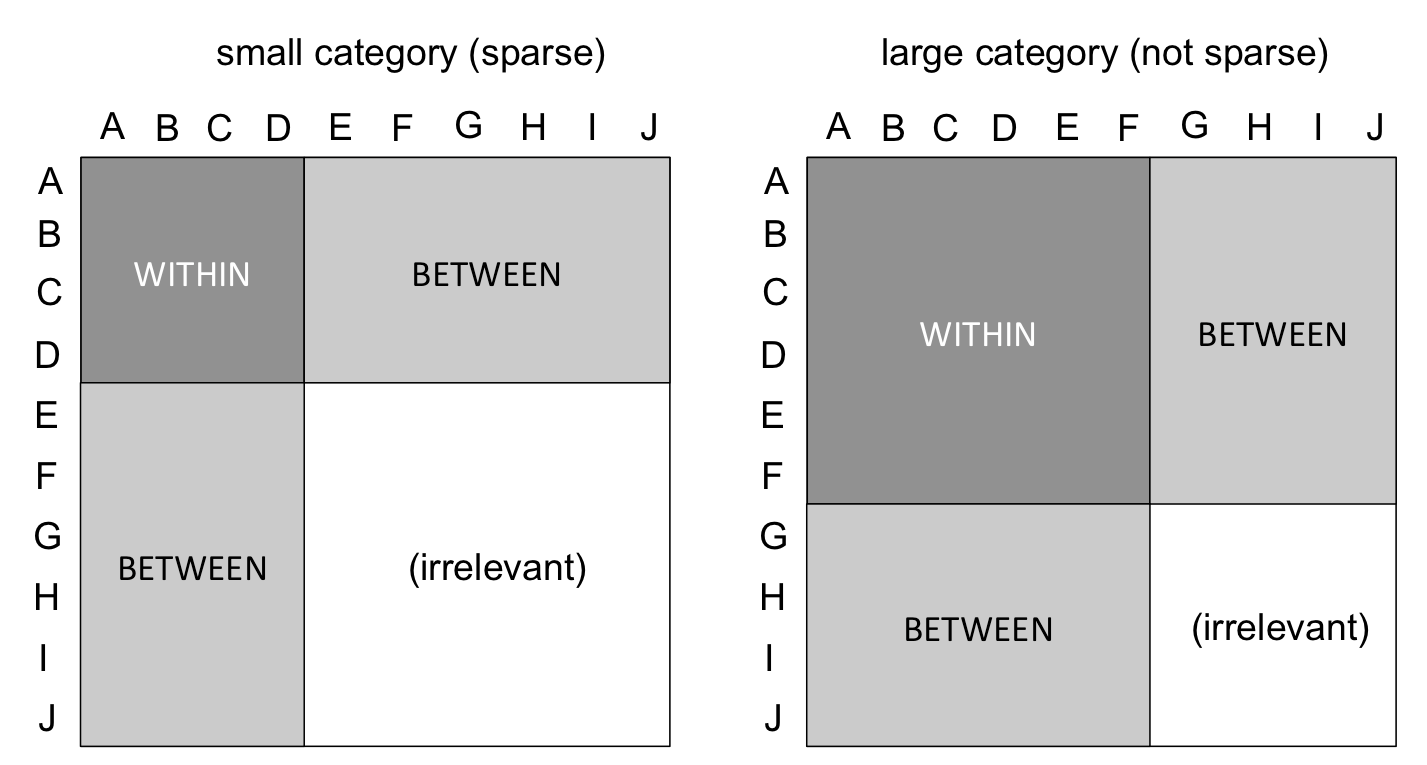
\epsfig{file=similarity.eps,width=12cm}
\caption{An illustration of which similarities contribute to the calculation of category goodness, for domain with $M=10$ items. On the left, we have a small category containing 4 items (A,B,C,D) and on the right the category is large, with 6 items (A,B,C,D,E,F). In both figures, the dark shaded area corresponds to elements of the similarity matrix that contribute to the calculation of the within-category similarity, whereas the lightly shaded areas indicate which pairwise similarities contribute to the between-category similarity. Unshaded areas make no contribution, and are hence irrelevant. The key observation is that larger categories implicate a much larger proportion of the matrix.} \label{simmatrix}
\end{center}
\end{figure}


%In these expressions, the pairwise similarity function $s(x_i,x_j)$ can be formalized in many ways; via distance in psychological space \cite{Attneave1950}, in terms of feature overlap \cite{Tversky1977}, or many other possibilities. All that matters for the current purposes is that some well-defined subjective similarity structure exists. As it turns out, we it is





%then we can use the family resemblance principle to define a formal measure of the ``goodness'' of that category, denoted $g_h$.

%With this in mind, we can define the goodness $g_h$ of some hypothesized rule $h$ as the average similarity among all pairs of items for which both items satisfy the rule (within-category) {\it minus} the average similarity among all pairs of items for which one satisfies the rule and one does not (between-category).

%To formalize this, let $\bm{x}^{(h)}$ denote the set of entities that are consistent with the rule $h$, and let $s(x_i,x_j)$ denote the similarity between entities $x_i$ and $x_j$. The pairwise similarity function $s(x_i,x_j)$ can be formalized in many way; via distance in psychological space \cite{Attneave1950}, in terms of feature overlap \cite{Tversky1977}, or many other possibilities. All that matters for the current purposes is that some well-defined subjective similarity structure exists. For a rule that is true for $m_h$ items, the average similarity among members is given by,
%%
%\begin{equation}
%S(h,h) = \frac{1}{m_h(m_h-1)}\sum_{x_i \in \bm{x}^{(h)}}  \sum_{x_j \in \bm{x}^{(h)}} s(x_i,x_j)
%\end{equation}
%%
%\noindent
%where the sum is taken over all $i \neq j$.  The average similarity between category members and non-members is accordingly
%%
%\begin{equation}
%S(h,1-h) = \frac{1}{2m_h (M-m_h)} \sum_{x_i \in \bm{x}^{(h)}} \sum_{x_j \notin \bm{x}^{(h)}} s(x_i,x_j).
%\end{equation}
%\noindent
%The goodness of the category is simply the difference between these two averages:
%%
%\begin{equation}
%g_h = S(h,h) - S(h,1-h).
%\end{equation}
%Thus, if $g_h>0$ then the entities within the category are more similar to each other than they are to other entities, and the category is a good one in the family resemblance sense. In contrast, if $g_h<0$, then the category members are actually more similar to non-members than they are to one another, and it is therefore a bad family resemblance category.

\begin{figure}[ph]
\begin{center}
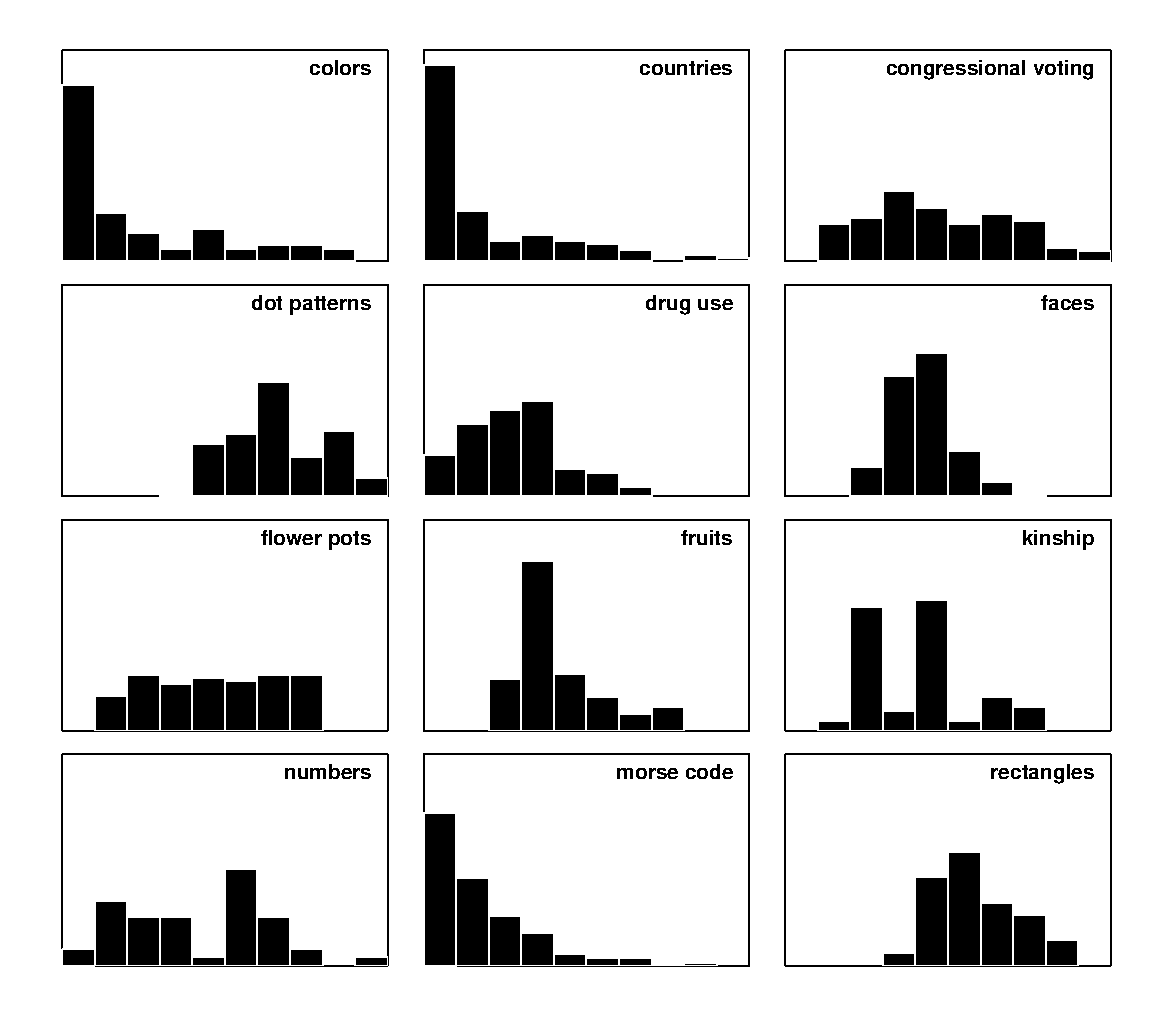
\epsfig{file=distributionofsimilarity.eps,width=12cm}
\caption{The marginal distribution over empirical similarities for several domains. All plots are drawn on the same scale, with the horizontal axis running from 0 to 1  since all data sets have been normalized so that similarities fall within this range. Across 12 data sets it is clear that similarities can be distributed in many different ways. The data sets are all available online courtesy of Michael Lee (\protect\url{www.socsci.uci.edu/~mdlee/sda.html}) and cover a range of collection methodologies and domains. Specifically the data relate to colors \protect\cite{Ekman1954}, countries \protect\cite{Navarro2002}, congressional voting patterns \protect\cite{Romesburg1984}, dot patterns \protect\cite{Glushko1975}, patterns of drug use \protect\cite{Huba1981}, photographs of faces (unpublished data, Michael Lee), drawings of flower pots \protect\cite{Gati1982}, fruits \protect\cite{Tversky1986}, kinship terms \protect\cite{Rosenberg1975}, the numbers 0-9 \protect\cite{Shepard1975}, morse code patterns \protect\cite{Rothkopf1957} and rectangles with interior line segments \protect\cite{Kruschke1993}.}
\label{distributionofsimilarity}
\end{center}
\end{figure}


%the kind of logical structure that underlies the similarities between entities -- that is, what type of mental representation (spaces, trees, partitions, features, etc) that gives rise to the similarity function $s(x_i,x_j)$ --

In what ways can the goodness of categories vary? Clearly, this depends in part on the precise nature of the pairwise similarity function $s(x_i,x_j)$. As such, there would be expected to be idiosyncratic variations across different stimulus domains. For instance, if similarities are constrained by a geometric structure \cite<e.g.>{Attneave1950}, we might expect somewhat different answers than would be obtained if similarities are described in terms of feature overlap \cite{Tversky1977}. However, we wish to argue that while some things are specific, and depend on the particular structure that underlies the similarity function, other there are {\it also} some regularities that might be expected to be universal (or nearly so), and do not actually depend on the details of the similarity structure. In particular, we suggest that sparsity is one such universal.

With this in mind, in our derivation below we strip out almost everything that might plausibly be called ``structure'' from the similarity function. In effect, we treat the pairwise similarities as if they were independent and identically distributed random variables. Moreover, since the (marginal) distribution of empirically-measured similarities varies wildly across domains (see Figure~\ref{distributionofsimilarity}) we make almost no assumptions about what distribution the pairwise similarities are generated from. The {\it only} constraint we impose is to assume that this distribution has finite mean and finite, non-zero variance. In other words, we assume that the pairwise similarities among entities are not all identical: there must be some variation in the world. The reason for taking this ``minimalist'' approach is as follows: our goal is to ensure that our derivation does not implicitly rely on any deeper representational structure, and thus show that sparsity follows from the family resemblance principle itself. The simplest way to do this is to remove any such structure. It should {\it not} be construed as a claim that no deeper structure exists in real life.


%} drawn from some unknown distribution. Since empirical similarities vary considerably in how they are distributed (see Figure~\ref{distributionofsimilarity}) our derivation assumes only that this distribution has finite mean and finite, non-zero variance. Applying these assumptions, we can use the central limit theorem to show that for a rule $h$ that is satisfied by $m_h$ items, the goodness of categories statistic $g_h$ is approximately normally distributed with mean 0 and variance that depends on the size of the category $m_h$:
%%

Given these extremely weak assumptions, what can we say abut the distribution of the category goodness measure $g_h$? While the raw distribution over {\it pairwise} similarities $s(x_i,x_j)$ can take any shape so long as it has finite mean $\mu$ and variance $\sigma^2$, the central limit theorem \cite<e.g.>[theorem B.97]{schervish95} implies that (in the limit) the within and between category {\it averages} become normally distributed
%%
\begin{eqnarray}
s_{\rm in}(\bm{x}_h) &\sim& \mbox{Normal}\left(\mu,\frac{\sigma^2}{m_h(m_h-1)}\right) \\
s_{\rm out}(\bm{x}_h) &\sim& \mbox{Normal}\left(\mu,\frac{\sigma^2}{2m_h (M-m_h)}\right).
\end{eqnarray}
%%
\noindent
However, the critical point here is not the fact that the distributions become normal, but rather the fact that the variance of these distributions depends on the number of items $m_h$ that belong to the category. Taking the difference between these variables yields the following asymptotic distribution for the category goodness measure:
%%
\begin{equation}
g_h \sim \mbox{Normal}\left( 0, \frac{\sigma^2}{m_h(m_h-1)} + \frac{\sigma^2}{2m_h (M-m_h)} \right).
\end{equation}
\noindent
Notice that the value of $\sigma$ just acts as a scaling constant and plays no role in determining the sparsity of the resulting hypothesis space. That is, if the combination $\sigma_1$, $\gamma_1$ yields an expected sparsity $\theta$, then for every other possible variance $\sigma_2$ there exists a corresponding threshold $\gamma_2$ that yields the same sparsity $\theta$. Conversely, if there is no value $\gamma_1$ that would yield sparsity $\theta$ if the variance is $\sigma_1$, then there is no value of $\gamma_2$ that would do so for $\sigma_2$. Thus, for simplicity and without loss of generality we set $\sigma=1$, which gives
\begin{equation}
g_h \sim \mbox{Normal}\left( 0, \frac{1}{m_h(m_h-1)} + \frac{1}{2m_h (M-m_h)} \right).
\label{goodness}
\end{equation}
Now, notice that the function that describes the variance of the distribution over category goodness
\begin{equation}
\frac{1}{m_h(m_h-1)} + \frac{1}{2m_h (M-m_h)}
\end{equation}
is largest when $m_h$ is small.\footnote{To be strictly accurate, this function is not perfectly monotonic. The minor violation of monotonicity is due to the fact that the category goodness calculation involves the difference between two averages (i.e., the within-category similarity and the between-category similarity), rather than a single average. As such, there is a minor violation of this effect that occurs when the rule in question is almost completely non-sparse (i.e., when $m_h \approx M$). However, as is clear from Figure~\ref{expectedsparsity} this weak violation of monotonicity does not induce a non-sparse hypothesis space.}
 The difference in variance means that it is ``easier'' to find a very good sparse rule than it is to find a very good non-sparse one. It also implies that it is easier to find a very bad sparse rule, but since the learner is presumably uninterested in finding bad rules, this is not particularly interesting.


This difference in variability emerges because sparser rules involve aggregating over fewer similarities.  To understand why, consider Figure~\ref{simmatrix}. It illustrates which cells in a $10 \times 10$ similarity matrix contribute to the category goodness calculation for a sparse category containing 4 objects (left) and non-sparse one containing 6 objects (right). The dark shaded area corresponds to elements of the similarity matrix that contribute to the calculation of the within-category similarity, whereas the lightly shaded areas indicate which pairwise similarities contribute to the between-category similarity. Unshaded areas make no contribution, and are hence irrelevant. Note that the rule indexing fewer items has many more unshaded cells, indicating that sparser rules involve fewer pairwise similarity calculations. What this means is that it is much easier to find a small collection of items that are especially similar to one another {\it or} especially dissimilar to one another. In essence, this is what the central limit theorem implies -- the more pairwise similarities that we have to average over to compute the category goodness, the more likely it is that the category will be ``average'' (i.e., have $g_h$ very close to zero).

The consequence of this is that the very best categories are sparse, as are the very worst ones. For instance, the numbers 2, 4 and 6 are much more similar to one another than most numbers, and so (2,4,6) is reasonably good category (i.e., $g_h > 0)$. In contrast, 0, 2 and 7 are unusually dissimilar, and so (0,2,7) ends up being a bad category (i.e., $g_h < 0$). However, when one looks at the complementary categories (0,1,3,5,7,8,9) and (1,3,4,5,6,8,9), it is clear that these are {\it both} mediocre at best ($g_h \approx 0$). In the first case, there are some items that are very similar (the five odd numbers) to one another, but since these are lumped in with two non-odd numbers (0 and 8) it is not a very good category. In the second case, there is a run of consecutive numbers from 3 to 6, but there are three other numbers in the category, so it too is fairly poor. That is, small categories have the potential to be very good and very bad, while large categories do not.

This is not unique to the numbers domain, of course. The small category {\textsc (mother, father, daughter, son)} is very sparse, and feels like a very good category (it has $g_h \gg0$) -- it is put together from kinship terms that are unusually similar to one another. In contrast, the small category (grandmother, uncle, cousin, brother) feels like a very bad category (it has $g_h \ll 0$) -- it is put together by choosing a deliberately weird grouping. The complementary categories in both cases consist of a large number of kinship terms, some of which are similar and others are not, and hence have $g_h \approx 0$ in both cases.



\subsection{Sparsity, finite memory and family resemblance}

What does this tell us about sparsity? To answer this, recall that in a domain with $M$ items, there are a total of $2^M$ distinct ways to group items together into a category. As the domain size becomes large, this number becomes so large that even a learner with a very large memory capacity will only be able to encode a small proportion of them. With this in mind, suppose that the learner retains only the best possible categories. Specifically, imagine that the learner has some threshold $\gamma$ such that the rule $h$ is an admissible member of $\ruleset$ only if the goodness $g_h$ is greater than that threshold. Notice that we place no particular {\it structural} constraints on which categories are included: for $\gamma>0$ the learner ends up with a collection of good categories that need not form a tree, a partition or any other structure. Using the result in Equation~\ref{goodness}, we can calculate the expected sparsity of the selected categories as a function of $\gamma$ (see Appendix for technical details). This function is plotted in the left panel of Figure~\ref{expectedsparsity} for a domain consisting of $M=16$ entities. As is clear from inspection, when the threshold is high enough ($\gamma>0$) the hypothesis space tends to be sparse (that is, $\theta < 1/2$); and as the threshold gets higher, the average sparsity decreases.

One natural question to ask is whether this pattern occurs for real data sets, since the simplifying assumptions that we have made (such as independence) will not necessarily hold, and the analysis makes use of an asymptotic argument based on the central limit theorem. There are many empirical similarity matrices that have been published, and so it is straightforward to verify that the prediction holds. Examples constructed from three empirical similarity matrices are shown in the right panel of Figure~\ref{expectedsparsity}. The numbers data is a similarity matrix that estimates the similarity between all pairs of numbers in the range 0-9 \cite{Shepard1975}. The kinship data \cite{Rosenberg1975} examines the perceived similarity between 15 different kinship relations (e.g., brother, sister, cousin, father). Finally, the numbers data measures the perceived similarity between 16 nations \cite{Navarro2002}. In each case, we calculated the goodness for all $2^M$ possible categories (where $M=10$ for numbers, $M=15$ for kinship and $M=16$ for countries), and then used these calculations to infer the sparsity $\theta$ that would emerge if the learner included only those categories with $g_h>\gamma$, for a range of $\gamma$ values. As is clear from inspection, the empirical data show the expected pattern. That is, good family resemblance categories tend to be sparse.


\begin{figure}
\begin{center}
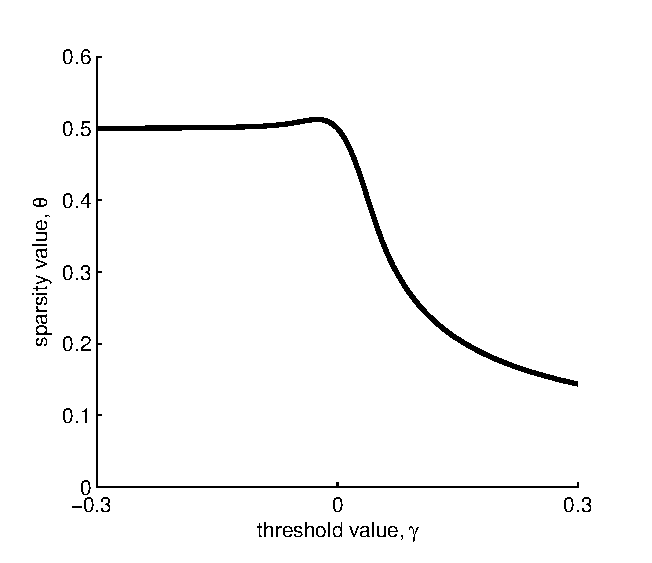
\epsfig{file=predictedsparsity_contrastmodel.eps,width=7cm}
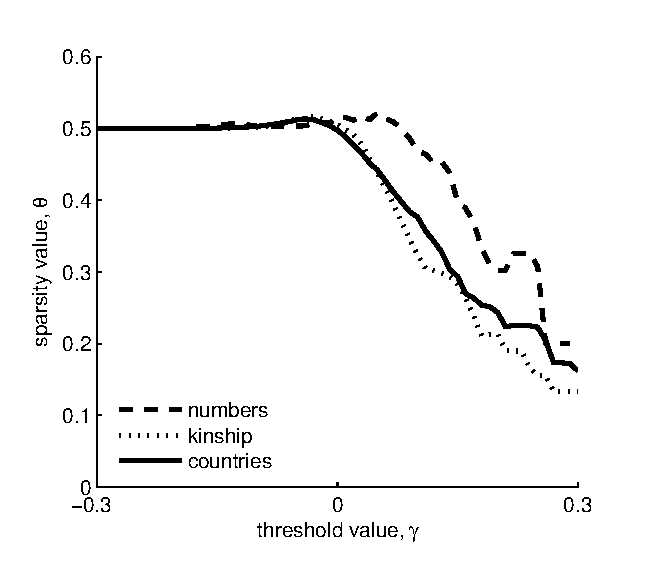
\epsfig{file=empiricalsparsity.eps,width=7cm}
\caption{On the left, the expected sparsity $\theta$ of the hypothesis space $\ruleset$ plotted as a function of the threshold $\gamma$, for a small domain with $M=16$ entities. On the right, the corresponding functions for three empirical data sets, numbers ($M=10$), kinship terms ($M=15$) and countries ($M=16)$.} \label{expectedsparsity}
\end{center}
\end{figure}


We can see this in a little more detail if we calculate the category goodness for all possible categories in some domain, and plot this as a function of size. Figure~\ref{rulethresholds} depicts the effects of three different choices of threshold $\gamma$ given all $2^{15}=32768$ logically possible categories for the kinship terms. The horizontal axis captures the number of entities $m_h$ captured by the rule while the vertical axis captures the goodness of the rule $g_h$. As predicted, the sparse rules vary widely in goodness, whereas less sparse ones are all close to the average. As a result, when $\gamma=0$, about half of the possible categories meet the threshold, and there is no sparsity bias in the corresponding hypothesis space $\ruleset$ (on average, the rules admitted into $\ruleset$ index 7.58 of the 15 items). However, when the threshold is raised (for instance, to $\gamma=0.15$ or $\gamma=0.075$), only the sparser rules are good enough to be included.

\begin{figure}
\begin{center}
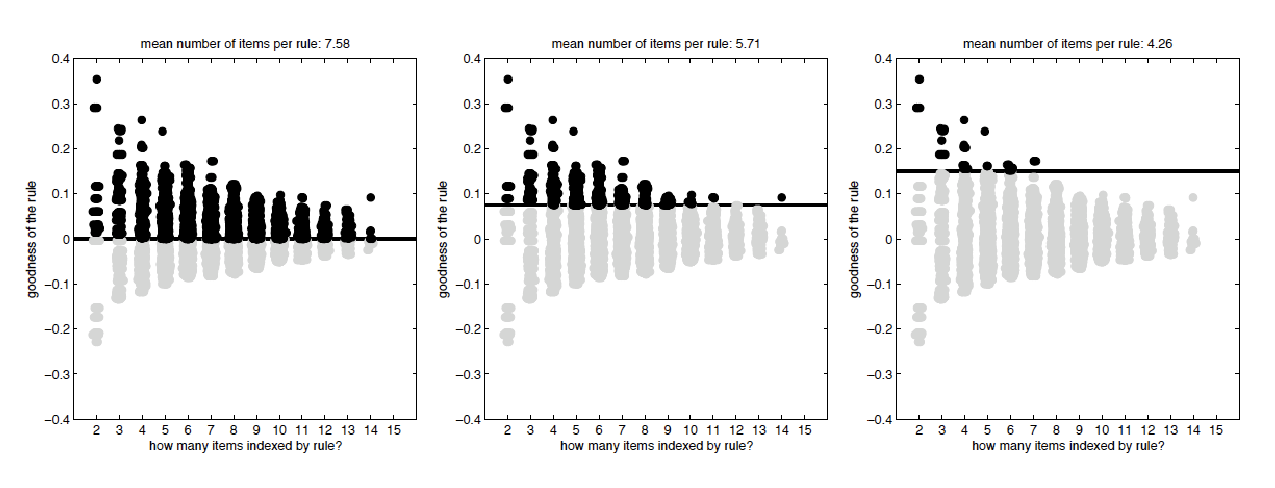
\epsfig{file=thresholds_lores.eps,width=15cm}
%\epsfig{file=threshold1.eps,width=5cm}
%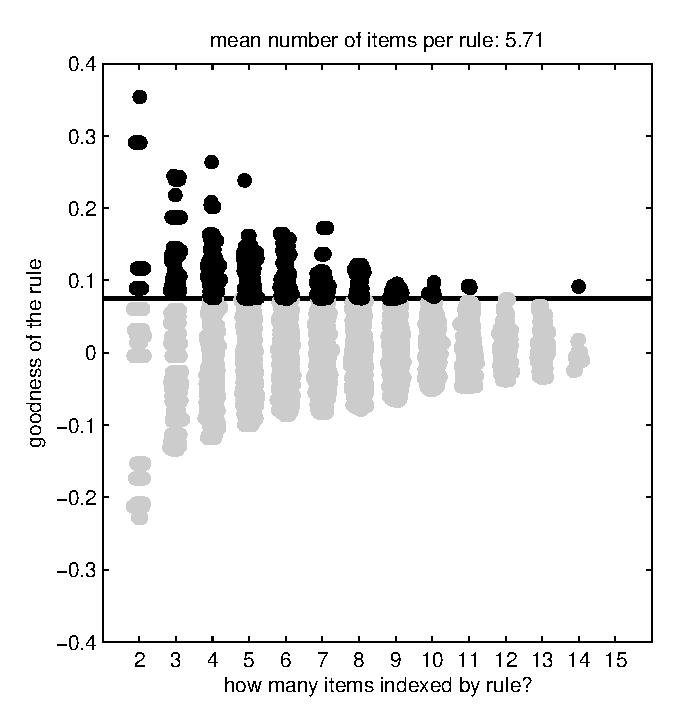
\epsfig{file=threshold2.eps,width=5cm}
%\epsfig{file=threshold3.eps,width=5cm}
\caption{Illustration of the emergence of a sparsity bias. Each panel plots both the size $m_h$ and goodness $g_h$ of all 32768 possible categories for the kinship data. The solid line depicts the threshold $\gamma$; black dots correspond to rules that meet the threshold, grey dots are those that do not. The overall triangular shape of the data is a consequence of the central limit theorem, and so when the learner imposes the requirement that the admissable rules be good (i.e., $\gamma>0$), a sparsity bias emerges.} \label{rulethresholds}
\end{center}
\end{figure}





% precisely by virtue of {\it being} good family resemblance categories.

% (numbers data from \citeNP{Shepard1975}, kinship data from \citeNP{Rosenberg1975}, and countries data from \citeNP{Navarro2002}). This is because the pattern is a mathematical consequence of the way that the goodness of a category is calculated and the requirement that the hypothesis space include only those rules that correspond to sufficiently good categories.


\section{Discussion}

The analysis presented in this paper is necessarily somewhat simplified. We therefore briefly discuss a range of issues that it raises and the assumptions upon which it relies.


\subsection{Structure in the world}

Perhaps the most obvious simplification in this paper is that we make very minimal assumptions about the structure of the world: we assume that some stimuli are more similar than others, but there is no other source of structure built into the analysis. We also assume that the rules admitted to $\ruleset$ are statistically independent of one another. Naturally, we expect that the real world is considerably more structured than these assumptions imply. This does not change our basic point, which is that only a very minimal amount of structure is actually {\it needed} to induce the sparsity bias and hence the PTS.

Nevertheless, it is interesting to consider in what ways the world might diverge from the assumptions we have made, and what this would mean for our analysis. Perhaps the most obvious point of divergence occurs when we relax the assumption that the rules are independent from one another.  In that case, it might be possible for the learner to acquire structured background knowledge that allows him to bypass the capacity constraints and therefore make better queries based on this knowledge.  When playing the everyday version of 20 questions, for instance, people typically start with ``animal/mineral/vegetable'' queries as a method for approximating globally optimal questions without explicitly representing the complete set of possible objects. In such cases it may be possible to improve on the positive test approach.  However, the original \citeA{wason60} task -- and many other typical situations, including scientific discovery -- makes such a strategy difficult: the set of plausible rules is too large to hold in working memory, and there is no easy way to use global domain knowledge or exploit dependencies among the rules. Our analysis suggests that it is precisely in such cases that the positive test strategy approaches optimality.

\subsection{Implicit falsification and the role of memory}

One question worth considering is the difference between falsifying the explicit rules in $\ruleset_E$ and those in the complementary set of {\it implicit} rules $\ruleset_I$. This issue is reminiscent of early discussions of the rule-discovery task \cite{Wetherick1962,Wason1962} in which a distinction was drawn between falsification of a hypothesis explicitly considered by a participant (falsification in $\ruleset_E$), and the kind of implicit falsification that occurs because the oracle's responses are inconsistent with a great many rules, regardless of whether the learner has explicitly considered them (falsification in $\ruleset_I$). The analysis in this paper treats both of these events as genuine falsifications, even though the learner would be unaware of implicit falsifications. The natural way in which this might happen is simply that these implicitly eliminated hypotheses are never considered, since they are inconsistent with previous observations. Nothing in the analysis requires learners to be aware of this, however; it merely requires that they not generate hypotheses that are inconsistent with the data so far.

Of course, this aspect of our analysis may be seen as a bit odd: why assume that the learner has limited memory capacity for hypotheses but perfect memory for the data? In many situations such an assumption is not unreasonable: for instance, it is trivially the case that data are easily ``remembered'' by virtue of being written down, whereas the complete set of logically possible hypotheses is almost never easily accessible.  In such cases there is a genuine asymmetry between data and hypotheses.  However, since such arrangements are by no means universal, it is instructive to consider how the analysis would change if we relaxed the assumption that data are perfectly remembered. Our conjecture is that the same qualitative pattern would emerge, with a positive test strategy converging on the correct rule more quickly than other strategies. The main difference would be that all strategies would learn more slowly. To see why this would be the case, suppose that we (rather simplistically) formalize the notion of limited memory by assuming that some data are randomly deleted from memory. This would effectively be the same as if that data had never been seen: any hypotheses that would have been eliminated by such data would no longer be treated as having been falsified.  However, since the analysis does not depend on any particular assumptions about what sort of data has or has not been seen, dropping data at random would not change the relative performance of different types of strategies. Only if the learner is more likely to forget data resulting from positive tests than negative tests would this analysis change; but if anything, the opposite assumption may be true \cite{taplin75}.

This does raise the broader question of what our approach presumes about the nature of memory. We assume that the learner constructs a space of plausible rules $\ruleset$, from which a small number of explicit hypotheses $\ruleset_E$ are selected and tested. One possible interpretation of such an assumption is that the larger hypothesis space $\ruleset$ might correspond to concepts that are activated in long-term memory, while the explicit hypotheses $\ruleset_E$ could correspond to the contents of working memory.  However, we stress that this interpretation is by no means critical to the analysis: we adopted this ``two-stage'' construction primarily so that we could analyze hypothesis generation and hypothesis testing as two distinct problems. Introducing the idea that $\ruleset$ corresponds to a set of ``plausible'' rules allowed us to show that $\ruleset$ tends to be sparse in an analysis distinct from demonstrating that the PTS follows from this sparsity. Yet this construction is rather artificial; for instance, we could consider a situation in which long term memory has access to all 32768 rules in Figure~\ref{rulethresholds} and generates explicit hypotheses $\ruleset_E$ directly, but with a strong bias to prefer good rules, or in such a way as to place a high prior probability over the best rules. This would produce a similar result, although the full story in this case is slightly more complex and is beyond the scope of this paper.

\subsection{Other extensions}

One of the respects in which our analysis is less general than that of \citeA{klaymanha87} is that we have addressed only the ``active learning'' situation where the learner chooses the query item and the oracle provides answers to the query. The natural counterpart to this scenario -- considered by \citeA{klaymanha87} but omitted here -- is ``observational learning'', where the oracle generates either positive evidence (consistent with the true rule) or negative evidence (inconsistent with the true rule). The main reason we do not discuss this situation is that there exists a considerable body of work that bears on this problem already. The Bayesian theory of generalization \cite{tenenbaumgriffiths01,sanjanatenenbaum02,navarroetal08} is strongly premised on the notion that natural concepts tend to be sparse phenomena, for which positive evidence is particularly powerful, and that people leverage off this to learn the meaning of words \cite{Xu2007} among other things. Similarly, recent research on ``pedagogical sampling'' suggests that learning in both adults and children is sensitive to the nature of the choices made by the oracle \cite{shaftogoodman08,bonawitzetal09}. And while early papers in computational learning theory seemed to suggest the children should not be able to learn languages from the positive-only evidence \cite{gold67}, more recent work \cite<e.g.,>{muggleton97,chatervitanyi07,perforsetal09} suggests that learning from positive evidence can be quite powerful. In view of this existing literature and the fact that the classic decision-making results \cite{wason60,wason68} relate primarily to the active learning scenario, we only discuss the active case in detail here.

Our analysis is also restricted to the rule-discovery problem. This problem is quite broad, covering a range of interesting problems in science, language learning and categorization, but there are other tasks that remain outside its scope. Most obviously, since our main goal was to consider the interaction between hypothesis generation and hypothesis testing, the link to the four-card selection task is complicated by the fact that it does not involve any hypothesis generation. This is not to say that there are no implications to be drawn, but in view of the fact that other analysis already cover the selection task in some detail \cite{oaksfordchater94} we do not address it here.

\subsection{Capacity limited rationality}

Since the analysis makes use of Bayesian theories of categorization \cite{Anderson1991,griffithssanborncanininavarro08}, hypothesis generation \cite{gettysfisher79} and hypothesis testing \cite{klaymanha87}, it should be clear that we have focused primarily on the optimal solution to the computational problem facing the learner \cite{marr82}, and not on the processes by which such solutions may be reached. Even so, our analysis differs from a ``standard'' computational level analysis \cite<e.g.>{shepard87,tenenbaumgriffiths01} since we assume that processing constraints (probably in the form of working memory) that place a limit on the number of hypotheses one can explicitly consider play a central role in explaining human behavior. Thus, ours is a rational analysis in the sense that we show that positive testing is a {\it conditionally} optimal search strategy for a learner who has to deal with those constraints. It is similar in spirit to the ``rational approximation'' idea proposed by \citeA{sanborngriffithsnavarro06} and the ``locally Bayesian learning'' idea considered by \citeA{krushcke06}. In fact, one way of characterizing the approach is as an attempt to incorporate architectural assumptions into rational analysis \cite<see>[for discussion]{anderson07}. As we conceive it, the working memory constraint on the size of $\mathcal{H}_E$ and the long term memory constraint on the size of $\mathcal{H}$ are properties of the underlying cognitive architecture. Rather than ignore these ideas when modeling human learning, we instead treat the core ideas (e.g., working memory constraints) as fixed and then seek to solve the relevant computational problem (rule learning) conditional on this architecture. The result is a kind of rational analysis that still deals with universal computational problems \cite{shepard87} but nevertheless is sensitive to the kinds of basic memory limitations \cite{miller56,cowan01} that might apply to real-world learners.

\section{Conclusion}

We demonstrate two findings in this paper. In the realm of hypothesis testing, we show that when rules are sparse and the learner has access only to a small number of hypotheses, the PTS tends to be the best learning method \cite<as in>{klaymanha87,oaksfordchater94}. In the realm of hypothesis generation, we suggest that sparse hypothesis spaces arise as a natural consequence of choosing sensible rules (this is implicit but not developed in some information-theoretic analyses, such as \citeA{cherubinietal05} and \citeA{Frank2009}).  While there is considerable existing evidence that people do represent the world sparsely, and the practical usefulness of sparse representations is evident in fields as diverse as machine learning, statistics, and neuroscience, we are not aware of any existing work that explicitly connects the two realms.

Taken together, the results provide a deeper theoretical explanation for the PTS. We envisage a learner who operates in a structured world and generates hypotheses in a Bayesian way \cite{gettysfisher79}, such that the prior over rules assigns higher probability to those rules that correspond to ``good'' family resemblance categories. Since good categories tend to be sparse, the learner tests them using the method that is optimal for sparse rules: the positive test strategy. Of course, this strategy is not perfect: no strategy can be when handling inductive problems, as the original \citeA{wason60} example illustrates. However, since the inevitability of inductive failures is considered to be a hard problem in philosophy \cite{hume1739,Goodman1955,goodman72}, scientific discovery \cite{feyerabend75} and computational learning \cite{Wolpert1997}, we might forgive human participants for following an optimal strategy that happens to fail in some cases.


\section{Acknowledgements}

Part of this work was presented at the 31st annual meeting of the Cognitive Science Society. DJN was supported by an Australian Research Fellowship (ARC grant DP0773794). We thank all of the people who commented on or reviewed the manuscript and the conference paper that it expands.

\bibliographystyle{apacite}



\begin{thebibliography}{}

\bibitem[\protect\citeauthoryear{%
Adsit%
\ \BBA{} London%
}{%
Adsit%
\ \BBA{} London%
}{%
{\protect\APACyear{1997}}%
}]{%
adsitlondon97}%
\APACinsertmetastar{%
adsitlondon97}%
Adsit, D.%
\BCBT{}\ \BBA{} London, M.%
%
\unskip\
\newblock
\APACrefYearMonthDay{1997}{}{}.
\newblock
\BBOQ{}\APACrefatitle{Effects of hypothesis generation on hypothesis testing in
  rule-discovery tasks}{Effects of hypothesis generation on hypothesis testing
  in rule-discovery tasks}.\BBCQ{}
\newblock
\APACjournalVolNumPages{The Journal of General Psychology}{124}{1}{19--34}.
\PrintBackRefs{\CurrentBib}

\bibitem[\protect\citeauthoryear{%
Anderson%
}{%
Anderson%
}{%
{\protect\APACyear{1991}}%
}]{%
Anderson1991}%
\APACinsertmetastar{%
Anderson1991}%
Anderson, J\BPBI R.%
%
\unskip\
\newblock
\APACrefYearMonthDay{1991}{}{}.
\newblock
\BBOQ{}\APACrefatitle{The adaptive nature of human categorization}{The adaptive
  nature of human categorization}.\BBCQ{}
\newblock
\APACjournalVolNumPages{Psychological Review}{98}{3}{409--429}.
\PrintBackRefs{\CurrentBib}

\bibitem[\protect\citeauthoryear{%
Anderson%
}{%
Anderson%
}{%
{\protect\APACyear{2007}}%
}]{%
anderson07}%
\APACinsertmetastar{%
anderson07}%
Anderson, J\BPBI R.%
%
\unskip\
\newblock
\APACrefYear{2007}.
\newblock
\APACrefbtitle{How can the human mind exist in the physical universe?}{How can
  the human mind exist in the physical universe?}
\newblock
\APACaddressPublisher{Oxford}{Oxford Univerity Press}.
\PrintBackRefs{\CurrentBib}

\bibitem[\protect\citeauthoryear{%
Ashby%
\ \BBA{} Gott%
}{%
Ashby%
\ \BBA{} Gott%
}{%
{\protect\APACyear{1988}}%
}]{%
Ashby1988}%
\APACinsertmetastar{%
Ashby1988}%
Ashby, F\BPBI G.%
\BCBT{}\ \BBA{} Gott, R\BPBI E.%
%
\unskip\
\newblock
\APACrefYearMonthDay{1988}{}{}.
\newblock
\BBOQ{}\APACrefatitle{Decision rules in the perception and categorization of
  multidimensional stimuli}{Decision rules in the perception and categorization
  of multidimensional stimuli}.\BBCQ{}
\newblock
\APACjournalVolNumPages{Journal of Experimental Psychology: Learning, Memory,
  and Cognition}{14}{}{33-53}.
\PrintBackRefs{\CurrentBib}

\bibitem[\protect\citeauthoryear{%
Attneave%
}{%
Attneave%
}{%
{\protect\APACyear{1950}}%
}]{%
Attneave1950}%
\APACinsertmetastar{%
Attneave1950}%
Attneave, F.%
%
\unskip\
\newblock
\APACrefYearMonthDay{1950}{}{}.
\newblock
\BBOQ{}\APACrefatitle{Dimensions of similarity}{Dimensions of
  similarity}.\BBCQ{}
\newblock
\APACjournalVolNumPages{American Journal of Psychology}{63}{}{546-554}.
\PrintBackRefs{\CurrentBib}

\bibitem[\protect\citeauthoryear{%
Austerweil%
\ \BBA{} Griffiths%
}{%
Austerweil%
\ \BBA{} Griffiths%
}{%
{\protect\APACyear{2008}}%
}]{%
austerweilgriffiths08}%
\APACinsertmetastar{%
austerweilgriffiths08}%
Austerweil, J.%
\BCBT{}\ \BBA{} Griffiths, T.%
%
\unskip\
\newblock
\APACrefYearMonthDay{2008}{}{}.
\newblock
\BBOQ{}\APACrefatitle{A rational analysis of confirmation with deterministic
  hypotheses}{A rational analysis of confirmation with deterministic
  hypotheses}.\BBCQ{}
\newblock
\APACjournalVolNumPages{Proceedings of the 30th {A}nnual {C}onference of the
  {C}ognitive {S}cience {S}ociety}{}{}{}.
\PrintBackRefs{\CurrentBib}

\bibitem[\protect\citeauthoryear{%
Bonawitz%
\ \protect\BOthers{.}}{%
Bonawitz%
\ \protect\BOthers{.}}{%
{\protect\APACyear{2009}}%
}]{%
bonawitzetal09}%
\APACinsertmetastar{%
bonawitzetal09}%
Bonawitz, L.%
, Shafto, P.%
, Gweon, H.%
, Chang, I.%
, Katz, S.%
\BCBL{}\ \BBA{} Schulz, L.%
%
\unskip\
\newblock
\APACrefYearMonthDay{2009}{}{}.
\newblock
\BBOQ{}\APACrefatitle{The double-edged sword of pedagogy: Modeling the effect
  of pedagogy on preschoolers' exploratory play}{The double-edged sword of
  pedagogy: Modeling the effect of pedagogy on preschoolers' exploratory
  play}.\BBCQ{}
\newblock
\APACjournalVolNumPages{Proceedings of the 31st Annual Conference of the
  Cognitive Science Society}{}{}{}.
\PrintBackRefs{\CurrentBib}

\bibitem[\protect\citeauthoryear{%
Brown%
}{%
Brown%
}{%
{\protect\APACyear{1974}}%
}]{%
brown74}%
\APACinsertmetastar{%
brown74}%
Brown, A\BPBI S.%
%
\unskip\
\newblock
\APACrefYearMonthDay{1974}{}{}.
\newblock
\BBOQ{}\APACrefatitle{Examination of hypothesis-sampling theory}{Examination of
  hypothesis-sampling theory}.\BBCQ{}
\newblock
\APACjournalVolNumPages{Psychological Bulletin}{81}{11}{773 - 790}.
\PrintBackRefs{\CurrentBib}

\bibitem[\protect\citeauthoryear{%
Bruner%
, Goodnow%
\BCBL{}\ \BBA{} Austin%
}{%
Bruner%
\ \protect\BOthers{.}}{%
{\protect\APACyear{1956}}%
}]{%
brunergoodnowaustin56}%
\APACinsertmetastar{%
brunergoodnowaustin56}%
Bruner, J\BPBI S.%
, Goodnow, J\BPBI J.%
\BCBL{}\ \BBA{} Austin, G\BPBI A.%
%
\unskip\
\newblock
\APACrefYear{1956}.
\newblock
\APACrefbtitle{A study of thinking}{A study of thinking}.
\newblock
\APACaddressPublisher{New York}{Wiley}.
\PrintBackRefs{\CurrentBib}

\bibitem[\protect\citeauthoryear{%
Chater%
\ \BBA{} Vit{\`a}nyi%
}{%
Chater%
\ \BBA{} Vit{\`a}nyi%
}{%
{\protect\APACyear{2007}}%
}]{%
chatervitanyi07}%
\APACinsertmetastar{%
chatervitanyi07}%
Chater, N.%
\BCBT{}\ \BBA{} Vit{\`a}nyi, P.%
%
\unskip\
\newblock
\APACrefYearMonthDay{2007}{}{}.
\newblock
\BBOQ{}\APACrefatitle{`{I}deal learning' of natural language: Positive results
  about learning from positive evidence}{`{I}deal learning' of natural
  language: Positive results about learning from positive evidence}.\BBCQ{}
\newblock
\APACjournalVolNumPages{Journal of Mathematical Psychology}{51}{3}{135--163}.
\PrintBackRefs{\CurrentBib}

\bibitem[\protect\citeauthoryear{%
Cheng%
\ \BBA{} Holyoak%
}{%
Cheng%
\ \BBA{} Holyoak%
}{%
{\protect\APACyear{1985}}%
}]{%
Cheng1985}%
\APACinsertmetastar{%
Cheng1985}%
Cheng, P\BPBI W.%
\BCBT{}\ \BBA{} Holyoak, K\BPBI J.%
%
\unskip\
\newblock
\APACrefYearMonthDay{1985}{}{}.
\newblock
\BBOQ{}\APACrefatitle{Causal reasoning schemas}{Causal reasoning
  schemas}.\BBCQ{}
\newblock
\APACjournalVolNumPages{Cognitive Psychology}{17}{}{391-416}.
\PrintBackRefs{\CurrentBib}

\bibitem[\protect\citeauthoryear{%
Cherubini%
, Castelvecchio%
\BCBL{}\ \BBA{} Cherubini%
}{%
Cherubini%
\ \protect\BOthers{.}}{%
{\protect\APACyear{2005}}%
}]{%
cherubinietal05}%
\APACinsertmetastar{%
cherubinietal05}%
Cherubini, P.%
, Castelvecchio, E.%
\BCBL{}\ \BBA{} Cherubini, A\BPBI M.%
%
\unskip\
\newblock
\APACrefYearMonthDay{2005}{}{}.
\newblock
\BBOQ{}\APACrefatitle{Generation of hypotheses in {W}ason's 2-4-6 task: An
  information theory approach}{Generation of hypotheses in {W}ason's 2-4-6
  task: An information theory approach}.\BBCQ{}
\newblock
\APACjournalVolNumPages{The Quarterly Journal of Experimental
  Psychology}{58A}{2}{309--332}.
\PrintBackRefs{\CurrentBib}

\bibitem[\protect\citeauthoryear{%
Chomsky%
}{%
Chomsky%
}{%
{\protect\APACyear{1957}}%
}]{%
chomsky57}%
\APACinsertmetastar{%
chomsky57}%
Chomsky, N.%
%
\unskip\
\newblock
\APACrefYear{1957}.
\newblock
\APACrefbtitle{Syntactic Structures}{Syntactic structures}.
\newblock
\APACaddressPublisher{Berlin}{Mouton}.
\PrintBackRefs{\CurrentBib}

\bibitem[\protect\citeauthoryear{%
Cosmides%
}{%
Cosmides%
}{%
{\protect\APACyear{1989}}%
}]{%
cosmides89}%
\APACinsertmetastar{%
cosmides89}%
Cosmides, L.%
%
\unskip\
\newblock
\APACrefYearMonthDay{1989}{}{}.
\newblock
\BBOQ{}\APACrefatitle{The logic of social exchange: Has natural selection
  shaped how humans reason? {S}tudies with the {W}ason selection task}{The
  logic of social exchange: Has natural selection shaped how humans reason?
  {S}tudies with the {W}ason selection task}.\BBCQ{}
\newblock
\APACjournalVolNumPages{Cognition}{34}{}{93--107}.
\PrintBackRefs{\CurrentBib}

\bibitem[\protect\citeauthoryear{%
Cowan%
}{%
Cowan%
}{%
{\protect\APACyear{2001}}%
}]{%
cowan01}%
\APACinsertmetastar{%
cowan01}%
Cowan, N.%
%
\unskip\
\newblock
\APACrefYearMonthDay{2001}{}{}.
\newblock
\BBOQ{}\APACrefatitle{The magical number 4 in short-term memory: A
  reconsideration of mental storage capacity}{The magical number 4 in
  short-term memory: A reconsideration of mental storage capacity}.\BBCQ{}
\newblock
\APACjournalVolNumPages{Behavioral and Brain Sciences}{24}{}{87-185}.
\PrintBackRefs{\CurrentBib}

\bibitem[\protect\citeauthoryear{%
{De Deyne}%
\ \protect\BOthers{.}}{%
{De Deyne}%
\ \protect\BOthers{.}}{%
{\protect\APACyear{2008}}%
}]{%
DeDeyne2008}%
\APACinsertmetastar{%
DeDeyne2008}%
{De Deyne}, S.%
, Verheyen, S.%
, Ameel, E.%
, Vanpaemel, W.%
, Dry, M.%
, Voorspoels, W.%
\BCBL{}\ \BOthersPeriod{.}%
\unskip\
\newblock
\APACrefYearMonthDay{2008}{}{}.
\newblock
\BBOQ{}\APACrefatitle{Exemplar by feature applicability matrices and other
  Dutch normative data for semantic concepts}{Exemplar by feature applicability
  matrices and other dutch normative data for semantic concepts}.\BBCQ{}
\newblock
\APACjournalVolNumPages{Behavior Research Methods}{40}{}{1030-1048}.
\PrintBackRefs{\CurrentBib}

\bibitem[\protect\citeauthoryear{%
Doherty%
, Mynatt%
, Tweney%
\BCBL{}\ \BBA{} Schiavo%
}{%
Doherty%
\ \protect\BOthers{.}}{%
{\protect\APACyear{1979}}%
}]{%
dohertyetal79}%
\APACinsertmetastar{%
dohertyetal79}%
Doherty, M.%
, Mynatt, C.%
, Tweney, R.%
\BCBL{}\ \BBA{} Schiavo, M.%
%
\unskip\
\newblock
\APACrefYearMonthDay{1979}{}{}.
\newblock
\BBOQ{}\APACrefatitle{Pseudodiagnosticity}{Pseudodiagnosticity}.\BBCQ{}
\newblock
\APACjournalVolNumPages{Acta Psychologica}{43}{}{111-121}.
\PrintBackRefs{\CurrentBib}

\bibitem[\protect\citeauthoryear{%
Dougherty%
\ \BBA{} Hunter%
}{%
Dougherty%
\ \BBA{} Hunter%
}{%
{\protect\APACyear{2003}}%
}]{%
dougherty03}%
\APACinsertmetastar{%
dougherty03}%
Dougherty, M.%
\BCBT{}\ \BBA{} Hunter, J.%
%
\unskip\
\newblock
\APACrefYearMonthDay{2003}{}{}.
\newblock
\BBOQ{}\APACrefatitle{Hypothesis generation, probability judgment, and
  individual differences in working memory capacity}{Hypothesis generation,
  probability judgment, and individual differences in working memory
  capacity}.\BBCQ{}
\newblock
\APACjournalVolNumPages{Acta Psychologica}{113}{3}{263 -- 282}.
\PrintBackRefs{\CurrentBib}

\bibitem[\protect\citeauthoryear{%
Dunbar%
}{%
Dunbar%
}{%
{\protect\APACyear{1993}}%
}]{%
dunbar93}%
\APACinsertmetastar{%
dunbar93}%
Dunbar, K.%
%
\unskip\
\newblock
\APACrefYearMonthDay{1993}{}{}.
\newblock
\BBOQ{}\APACrefatitle{Concept discovery in a scientific domain}{Concept
  discovery in a scientific domain}.\BBCQ{}
\newblock
\APACjournalVolNumPages{Cognitive Science}{17}{}{397--434}.
\PrintBackRefs{\CurrentBib}

\bibitem[\protect\citeauthoryear{%
Ekman%
}{%
Ekman%
}{%
{\protect\APACyear{1954}}%
}]{%
Ekman1954}%
\APACinsertmetastar{%
Ekman1954}%
Ekman, G.%
%
\unskip\
\newblock
\APACrefYearMonthDay{1954}{}{}.
\newblock
\BBOQ{}\APACrefatitle{Dimensions of color vision}{Dimensions of color
  vision}.\BBCQ{}
\newblock
\APACjournalVolNumPages{Journal of Psychology}{38}{}{467-474}.
\PrintBackRefs{\CurrentBib}

\bibitem[\protect\citeauthoryear{%
Erickson%
\ \BBA{} Kruschke%
}{%
Erickson%
\ \BBA{} Kruschke%
}{%
{\protect\APACyear{1998}}%
}]{%
Erickson1998}%
\APACinsertmetastar{%
Erickson1998}%
Erickson, M\BPBI A.%
\BCBT{}\ \BBA{} Kruschke, J\BPBI K.%
%
\unskip\
\newblock
\APACrefYearMonthDay{1998}{}{}.
\newblock
\BBOQ{}\APACrefatitle{Rules and Exemplars in Category Learning}{Rules and
  exemplars in category learning}.\BBCQ{}
\newblock
\APACjournalVolNumPages{Journal of Experimental Psychology:
  General}{127}{}{107-140}.
\PrintBackRefs{\CurrentBib}

\bibitem[\protect\citeauthoryear{%
Evans%
}{%
Evans%
}{%
{\protect\APACyear{1972}}%
}]{%
evans1972}%
\APACinsertmetastar{%
evans1972}%
Evans, J\BPBI S\BPBI B\BPBI T.%
%
\unskip\
\newblock
\APACrefYearMonthDay{1972}{}{}.
\newblock
\BBOQ{}\APACrefatitle{Interpretation and `matching bias' in a reasoning
  task}{Interpretation and `matching bias' in a reasoning task}.\BBCQ{}
\newblock
\APACjournalVolNumPages{Quarterly Journal of Experimental
  Psychology}{24}{}{193-199}.
\PrintBackRefs{\CurrentBib}

\bibitem[\protect\citeauthoryear{%
Evans%
}{%
Evans%
}{%
{\protect\APACyear{1998}}%
}]{%
Evans1998}%
\APACinsertmetastar{%
Evans1998}%
Evans, J\BPBI S\BPBI B\BPBI T.%
%
\unskip\
\newblock
\APACrefYearMonthDay{1998}{}{}.
\newblock
\BBOQ{}\APACrefatitle{Matching bias in conditional reasoning: Do we understand
  it after 25 years?}{Matching bias in conditional reasoning: Do we understand
  it after 25 years?}\BBCQ{}
\newblock
\APACjournalVolNumPages{Thinking and Reasoning}{4}{}{45--82}.
\PrintBackRefs{\CurrentBib}

\bibitem[\protect\citeauthoryear{%
Evans%
\ \BBA{} Lynch%
}{%
Evans%
\ \BBA{} Lynch%
}{%
{\protect\APACyear{1973}}%
}]{%
evanslynch73}%
\APACinsertmetastar{%
evanslynch73}%
Evans, J\BPBI S\BPBI B\BPBI T.%
\BCBT{}\ \BBA{} Lynch, J.%
%
\unskip\
\newblock
\APACrefYearMonthDay{1973}{}{}.
\newblock
\BBOQ{}\APACrefatitle{Matching bias in the selection task}{Matching bias in the
  selection task}.\BBCQ{}
\newblock
\APACjournalVolNumPages{British Journal of Psychology}{64}{}{391--397}.
\PrintBackRefs{\CurrentBib}

\bibitem[\protect\citeauthoryear{%
Farris%
\ \BBA{} Revlin%
}{%
Farris%
\ \BBA{} Revlin%
}{%
{\protect\APACyear{1989}}%
}]{%
farrisrevlin89}%
\APACinsertmetastar{%
farrisrevlin89}%
Farris, H.%
\BCBT{}\ \BBA{} Revlin, R.%
%
\unskip\
\newblock
\APACrefYearMonthDay{1989}{}{}.
\newblock
\BBOQ{}\APACrefatitle{Sensible reasoning in two tasks: Rule discovery and
  hypothesis evaluation}{Sensible reasoning in two tasks: Rule discovery and
  hypothesis evaluation}.\BBCQ{}
\newblock
\APACjournalVolNumPages{Memory and Cognition}{17}{2}{221-232}.
\PrintBackRefs{\CurrentBib}

\bibitem[\protect\citeauthoryear{%
Feyerabend%
}{%
Feyerabend%
}{%
{\protect\APACyear{1975}}%
}]{%
feyerabend75}%
\APACinsertmetastar{%
feyerabend75}%
Feyerabend, P.%
%
\unskip\
\newblock
\APACrefYear{1975}.
\newblock
\APACrefbtitle{Against Method}{Against method}.
\newblock
\APACaddressPublisher{London}{New Left Books}.
\PrintBackRefs{\CurrentBib}

\bibitem[\protect\citeauthoryear{%
Frank%
, Goodman%
, Lai%
\BCBL{}\ \BBA{} Tenenbaum%
}{%
Frank%
\ \protect\BOthers{.}}{%
{\protect\APACyear{2009}}%
}]{%
Frank2009}%
\APACinsertmetastar{%
Frank2009}%
Frank, M\BPBI C.%
, Goodman, N\BPBI D.%
, Lai, P.%
\BCBL{}\ \BBA{} Tenenbaum, J\BPBI B.%
%
\unskip\
\newblock
\APACrefYearMonthDay{2009}{}{}.
\newblock
\BBOQ{}\APACrefatitle{Informative Communication in Word Production and Word
  Learning}{Informative communication in word production and word
  learning}.\BBCQ{}
\newblock
\APACjournalVolNumPages{Proceedings of the 31st Annual Conference of the
  Cognitive Science Society}{}{}{}.
\PrintBackRefs{\CurrentBib}

\bibitem[\protect\citeauthoryear{%
Freedman%
}{%
Freedman%
}{%
{\protect\APACyear{1992}}%
}]{%
freedman92}%
\APACinsertmetastar{%
freedman92}%
Freedman, E.%
%
\unskip\
\newblock
\APACrefYearMonthDay{1992}{}{}.
\newblock
\BBOQ{}\APACrefatitle{Scientific induction: Individual versus group processes
  and multiple hypotheses}{Scientific induction: Individual versus group
  processes and multiple hypotheses}.\BBCQ{}
\newblock
\APACjournalVolNumPages{Proceedings of the 14th Annual Conference of the
  Cognitive Science Society}{}{}{183--188}.
\PrintBackRefs{\CurrentBib}

\bibitem[\protect\citeauthoryear{%
Gati%
\ \BBA{} Tversky%
}{%
Gati%
\ \BBA{} Tversky%
}{%
{\protect\APACyear{1982}}%
}]{%
Gati1982}%
\APACinsertmetastar{%
Gati1982}%
Gati, I.%
\BCBT{}\ \BBA{} Tversky, A.%
%
\unskip\
\newblock
\APACrefYearMonthDay{1982}{}{}.
\newblock
\BBOQ{}\APACrefatitle{Representations of qualitative and quantitative
  dimensions}{Representations of qualitative and quantitative
  dimensions}.\BBCQ{}
\newblock
\APACjournalVolNumPages{Journal of Experimental Psychology: Human Perception
  and Performance}{8}{}{325-340}.
\PrintBackRefs{\CurrentBib}

\bibitem[\protect\citeauthoryear{%
Gettys%
\ \BBA{} Fisher%
}{%
Gettys%
\ \BBA{} Fisher%
}{%
{\protect\APACyear{1979}}%
}]{%
gettysfisher79}%
\APACinsertmetastar{%
gettysfisher79}%
Gettys, C\BPBI F.%
\BCBT{}\ \BBA{} Fisher, S\BPBI D.%
%
\unskip\
\newblock
\APACrefYearMonthDay{1979}{}{}.
\newblock
\BBOQ{}\APACrefatitle{Hypothesis plausibility and hypothesis
  generation}{Hypothesis plausibility and hypothesis generation}.\BBCQ{}
\newblock
\APACjournalVolNumPages{Organizational Behavior and Human
  Performance}{24}{}{93--110}.
\PrintBackRefs{\CurrentBib}

\bibitem[\protect\citeauthoryear{%
Gettys%
, Mehle%
\BCBL{}\ \BBA{} Fisher%
}{%
Gettys%
\ \protect\BOthers{.}}{%
{\protect\APACyear{1986}}%
}]{%
gettysmehlefisher86}%
\APACinsertmetastar{%
gettysmehlefisher86}%
Gettys, C\BPBI F.%
, Mehle, T.%
\BCBL{}\ \BBA{} Fisher, S.%
%
\unskip\
\newblock
\APACrefYearMonthDay{1986}{}{}.
\newblock
\BBOQ{}\APACrefatitle{Plausibility assessments in hypothesis
  generation}{Plausibility assessments in hypothesis generation}.\BBCQ{}
\newblock
\APACjournalVolNumPages{Organizational Behavior and Human Decision
  Processes}{37}{1}{14 - 33}.
\PrintBackRefs{\CurrentBib}

\bibitem[\protect\citeauthoryear{%
Glushko%
}{%
Glushko%
}{%
{\protect\APACyear{1975}}%
}]{%
Glushko1975}%
\APACinsertmetastar{%
Glushko1975}%
Glushko, R\BPBI J.%
%
\unskip\
\newblock
\APACrefYearMonthDay{1975}{}{}.
\newblock
\BBOQ{}\APACrefatitle{Pattern goodness and redundancy revisited:
  {M}ultidimensional scaling and hierarchical cluster analysis}{Pattern
  goodness and redundancy revisited: {M}ultidimensional scaling and
  hierarchical cluster analysis}.\BBCQ{}
\newblock
\APACjournalVolNumPages{Perception and Psychophysics}{17}{}{158-162}.
\PrintBackRefs{\CurrentBib}

\bibitem[\protect\citeauthoryear{%
Gold%
}{%
Gold%
}{%
{\protect\APACyear{1967}}%
}]{%
gold67}%
\APACinsertmetastar{%
gold67}%
Gold, E\BPBI M.%
%
\unskip\
\newblock
\APACrefYearMonthDay{1967}{}{}.
\newblock
\BBOQ{}\APACrefatitle{Language identification in the limit}{Language
  identification in the limit}.\BBCQ{}
\newblock
\APACjournalVolNumPages{Information and Control}{10}{}{447-474}.
\PrintBackRefs{\CurrentBib}

\bibitem[\protect\citeauthoryear{%
Goodman%
}{%
Goodman%
}{%
{\protect\APACyear{1955}}%
}]{%
Goodman1955}%
\APACinsertmetastar{%
Goodman1955}%
Goodman, N.%
%
\unskip\
\newblock
\APACrefYear{1955}.
\newblock
\APACrefbtitle{Fact, fiction, and forecast}{Fact, fiction, and forecast}.
\newblock
\APACaddressPublisher{Cambridge, MA}{Harvard University Press}.
\PrintBackRefs{\CurrentBib}

\bibitem[\protect\citeauthoryear{%
Goodman%
}{%
Goodman%
}{%
{\protect\APACyear{1972}}%
}]{%
goodman72}%
\APACinsertmetastar{%
goodman72}%
Goodman, N.%
%
\unskip\
\newblock
\APACrefYear{1972}.
\newblock
\APACrefbtitle{Problems and projects}{Problems and projects}.
\newblock
\APACaddressPublisher{}{Bobbs-Merrill}.
\PrintBackRefs{\CurrentBib}

\bibitem[\protect\citeauthoryear{%
Goodman%
, Tenenbaum%
, Feldman%
\BCBL{}\ \BBA{} Griffiths%
}{%
Goodman%
\ \protect\BOthers{.}}{%
{\protect\APACyear{2008}}%
}]{%
goodmanetal08}%
\APACinsertmetastar{%
goodmanetal08}%
Goodman, N.%
, Tenenbaum, J.%
, Feldman, J.%
\BCBL{}\ \BBA{} Griffiths, T.%
%
\unskip\
\newblock
\APACrefYearMonthDay{2008}{}{}.
\newblock
\BBOQ{}\APACrefatitle{A rational analysis of rule-based concept learning}{A
  rational analysis of rule-based concept learning}.\BBCQ{}
\newblock
\APACjournalVolNumPages{Cognitive Science}{32}{1}{108--154}.
\PrintBackRefs{\CurrentBib}

\bibitem[\protect\citeauthoryear{%
Goodnow%
\ \BBA{} Pettigrew%
}{%
Goodnow%
\ \BBA{} Pettigrew%
}{%
{\protect\APACyear{1955}}%
}]{%
Goodnow1955}%
\APACinsertmetastar{%
Goodnow1955}%
Goodnow, J\BPBI J.%
\BCBT{}\ \BBA{} Pettigrew, T.%
%
\unskip\
\newblock
\APACrefYearMonthDay{1955}{}{}.
\newblock
\BBOQ{}\APACrefatitle{Effect of prior patterns of experience upon strategies
  and learning sets}{Effect of prior patterns of experience upon strategies and
  learning sets}.\BBCQ{}
\newblock
\APACjournalVolNumPages{Journal of Experimental Psychology}{49}{}{381-389}.
\PrintBackRefs{\CurrentBib}

\bibitem[\protect\citeauthoryear{%
Gordon%
}{%
Gordon%
}{%
{\protect\APACyear{1999}}%
}]{%
Gordon1999}%
\APACinsertmetastar{%
Gordon1999}%
Gordon, A\BPBI D.%
%
\unskip\
\newblock
\APACrefYear{1999}.
\newblock
\APACrefbtitle{Classification}{Classification}\ (\PrintOrdinal{2nd}\ \BEd).
\newblock
\APACaddressPublisher{Boca Raton, FL}{Chapman and Hall}.
\PrintBackRefs{\CurrentBib}

\bibitem[\protect\citeauthoryear{%
Griffiths%
, Sanborn%
, Canini%
\BCBL{}\ \BBA{} Navarro%
}{%
Griffiths%
\ \protect\BOthers{.}}{%
{\protect\APACyear{2008}}%
}]{%
griffithssanborncanininavarro08}%
\APACinsertmetastar{%
griffithssanborncanininavarro08}%
Griffiths, T\BPBI L.%
, Sanborn, A\BPBI N.%
, Canini, K\BPBI R.%
\BCBL{}\ \BBA{} Navarro, D\BPBI J.%
%
\unskip\
\newblock
\APACrefYearMonthDay{2008}{}{}.
\newblock
\BBOQ{}\APACrefatitle{Categorization as nonparametric {B}ayesian density
  estimation}{Categorization as nonparametric {B}ayesian density
  estimation}.\BBCQ{}
\newblock
\BIn{} M.~Oaksford\ \BBA{} N.~Chater\ (\BEDS), \APACrefbtitle{The Probabilistic
  Mind: Prospects for {B}ayesian {C}ognitive {S}cience}{The probabilistic mind:
  Prospects for {B}ayesian {C}ognitive {S}cience}\ (\BPGS\ 303--328).
\newblock
\APACaddressPublisher{Oxford}{Oxford University Press}.
\PrintBackRefs{\CurrentBib}

\bibitem[\protect\citeauthoryear{%
Huba%
, Wingard%
\BCBL{}\ \BBA{} Bentler%
}{%
Huba%
\ \protect\BOthers{.}}{%
{\protect\APACyear{1981}}%
}]{%
Huba1981}%
\APACinsertmetastar{%
Huba1981}%
Huba, G\BPBI L.%
, Wingard, J\BPBI A.%
\BCBL{}\ \BBA{} Bentler, P\BPBI M.%
%
\unskip\
\newblock
\APACrefYearMonthDay{1981}{}{}.
\newblock
\BBOQ{}\APACrefatitle{A comparison of two latent variable causal models for
  adolescent drug use}{A comparison of two latent variable causal models for
  adolescent drug use}.\BBCQ{}
\newblock
\APACjournalVolNumPages{Journal of Personality and Social
  Psychology}{40}{1}{180-193}.
\PrintBackRefs{\CurrentBib}

\bibitem[\protect\citeauthoryear{%
Hume%
}{%
Hume%
}{%
{\protect\APACyear{1739/1898}}%
}]{%
hume1739}%
\APACinsertmetastar{%
hume1739}%
Hume, D.%
%
\unskip\
\newblock
\APACrefYear{1739/1898}.
\newblock
\APACrefbtitle{A Treatise of Human Nature}{A treatise of human nature}.
\newblock
\APACaddressPublisher{London}{Ward Lock}.
\PrintBackRefs{\CurrentBib}

\bibitem[\protect\citeauthoryear{%
Johnson-Laird%
, Legrenzi%
\BCBL{}\ \BBA{} Legrenzi%
}{%
Johnson-Laird%
\ \protect\BOthers{.}}{%
{\protect\APACyear{1972}}%
}]{%
Johnsonlaird1972}%
\APACinsertmetastar{%
Johnsonlaird1972}%
Johnson-Laird, P.%
, Legrenzi, P.%
\BCBL{}\ \BBA{} Legrenzi, M\BPBI S.%
%
\unskip\
\newblock
\APACrefYearMonthDay{1972}{}{}.
\newblock
\BBOQ{}\APACrefatitle{Reasoning and a sense of reality}{Reasoning and a sense
  of reality}.\BBCQ{}
\newblock
\APACjournalVolNumPages{British Journal of Psychology}{63}{}{395-400}.
\PrintBackRefs{\CurrentBib}

\bibitem[\protect\citeauthoryear{%
Johnson-Laird%
\ \BBA{} Wason%
}{%
Johnson-Laird%
\ \BBA{} Wason%
}{%
{\protect\APACyear{1970}}%
}]{%
johnsonlairdwason70}%
\APACinsertmetastar{%
johnsonlairdwason70}%
Johnson-Laird, P.%
\BCBT{}\ \BBA{} Wason, P.%
%
\unskip\
\newblock
\APACrefYearMonthDay{1970}{}{}.
\newblock
\BBOQ{}\APACrefatitle{A theoretical analysis of insight into a reasoning
  task}{A theoretical analysis of insight into a reasoning task}.\BBCQ{}
\newblock
\APACjournalVolNumPages{Cognitive Psychology}{1}{2}{134--148}.
\PrintBackRefs{\CurrentBib}

\bibitem[\protect\citeauthoryear{%
Jones%
\ \BBA{} Sugden%
}{%
Jones%
\ \BBA{} Sugden%
}{%
{\protect\APACyear{2001}}%
}]{%
Jones2001}%
\APACinsertmetastar{%
Jones2001}%
Jones, M.%
\BCBT{}\ \BBA{} Sugden, R.%
%
\unskip\
\newblock
\APACrefYearMonthDay{2001}{}{}.
\newblock
\BBOQ{}\APACrefatitle{Positive confirmation bias in the acquisition of
  information}{Positive confirmation bias in the acquisition of
  information}.\BBCQ{}
\newblock
\APACjournalVolNumPages{Theory and Decision}{50}{}{59-99}.
\PrintBackRefs{\CurrentBib}

\bibitem[\protect\citeauthoryear{%
Kemp%
\ \BBA{} Tenenbaum%
}{%
Kemp%
\ \BBA{} Tenenbaum%
}{%
{\protect\APACyear{2008}}%
}]{%
kemptenenbaum08}%
\APACinsertmetastar{%
kemptenenbaum08}%
Kemp, C.%
\BCBT{}\ \BBA{} Tenenbaum, J\BPBI B.%
%
\unskip\
\newblock
\APACrefYearMonthDay{2008}{}{}.
\newblock
\BBOQ{}\APACrefatitle{The discovery of structural form}{The discovery of
  structural form}.\BBCQ{}
\newblock
\APACjournalVolNumPages{Proceedings of the National Academy of
  Sciences}{105}{}{10687--10692}.
\PrintBackRefs{\CurrentBib}

\bibitem[\protect\citeauthoryear{%
Klahr%
\ \BBA{} Dunbar%
}{%
Klahr%
\ \BBA{} Dunbar%
}{%
{\protect\APACyear{1988}}%
}]{%
klahrdunbar88}%
\APACinsertmetastar{%
klahrdunbar88}%
Klahr, D.%
\BCBT{}\ \BBA{} Dunbar, K.%
%
\unskip\
\newblock
\APACrefYearMonthDay{1988}{}{}.
\newblock
\BBOQ{}\APACrefatitle{Dual space search during scientific reasoning}{Dual space
  search during scientific reasoning}.\BBCQ{}
\newblock
\APACjournalVolNumPages{Cognitive Science}{12}{}{1--48}.
\PrintBackRefs{\CurrentBib}

\bibitem[\protect\citeauthoryear{%
Klayman%
\ \BBA{} Ha%
}{%
Klayman%
\ \BBA{} Ha%
}{%
{\protect\APACyear{1987}}%
}]{%
klaymanha87}%
\APACinsertmetastar{%
klaymanha87}%
Klayman, J.%
\BCBT{}\ \BBA{} Ha, Y\BHBI W.%
%
\unskip\
\newblock
\APACrefYearMonthDay{1987}{}{}.
\newblock
\BBOQ{}\APACrefatitle{Confirmation, disconfirmation, and information in
  hypothesis testing}{Confirmation, disconfirmation, and information in
  hypothesis testing}.\BBCQ{}
\newblock
\APACjournalVolNumPages{Psychological Review}{94}{}{211-228}.
\PrintBackRefs{\CurrentBib}

\bibitem[\protect\citeauthoryear{%
Klayman%
\ \BBA{} Ha%
}{%
Klayman%
\ \BBA{} Ha%
}{%
{\protect\APACyear{1989}}%
}]{%
klaymanha89}%
\APACinsertmetastar{%
klaymanha89}%
Klayman, J.%
\BCBT{}\ \BBA{} Ha, Y\BHBI W.%
%
\unskip\
\newblock
\APACrefYearMonthDay{1989}{}{}.
\newblock
\BBOQ{}\APACrefatitle{Hypothesis testing in rule discovery: Strategy,
  structure, and content}{Hypothesis testing in rule discovery: Strategy,
  structure, and content}.\BBCQ{}
\newblock
\APACjournalVolNumPages{Journal of Experimental Psychology: Learning, Memory,
  and Cognition}{15}{4}{596--604}.
\PrintBackRefs{\CurrentBib}

\bibitem[\protect\citeauthoryear{%
Koehler%
}{%
Koehler%
}{%
{\protect\APACyear{1994}}%
}]{%
koehler94}%
\APACinsertmetastar{%
koehler94}%
Koehler, D\BPBI J.%
%
\unskip\
\newblock
\APACrefYearMonthDay{1994}{}{}.
\newblock
\BBOQ{}\APACrefatitle{Hypothesis Generation and Confidence in
  Judgment}{Hypothesis generation and confidence in judgment}.\BBCQ{}
\newblock
\APACjournalVolNumPages{Journal of Experimental Psychology: Learning, Memory,
  and Cognition}{20}{2}{461 - 469}.
\PrintBackRefs{\CurrentBib}

\bibitem[\protect\citeauthoryear{%
Kruschke%
}{%
Kruschke%
}{%
{\protect\APACyear{1992}}%
}]{%
Kruschke1992}%
\APACinsertmetastar{%
Kruschke1992}%
Kruschke, J\BPBI K.%
%
\unskip\
\newblock
\APACrefYearMonthDay{1992}{}{}.
\newblock
\BBOQ{}\APACrefatitle{{ALCOVE}: An exemplar-based connectionist model of
  category learning}{{ALCOVE}: An exemplar-based connectionist model of
  category learning}.\BBCQ{}
\newblock
\APACjournalVolNumPages{Psychological Review}{99}{1}{22-44}.
\PrintBackRefs{\CurrentBib}

\bibitem[\protect\citeauthoryear{%
Kruschke%
}{%
Kruschke%
}{%
{\protect\APACyear{1993}}%
}]{%
Kruschke1993}%
\APACinsertmetastar{%
Kruschke1993}%
Kruschke, J\BPBI K.%
%
\unskip\
\newblock
\APACrefYearMonthDay{1993}{}{}.
\newblock
\BBOQ{}\APACrefatitle{Human category learning: {I}mplications for
  backpropagation models.}{Human category learning: {I}mplications for
  backpropagation models.}\BBCQ{}
\newblock
\APACjournalVolNumPages{Connection Science}{5}{}{3-36}.
\PrintBackRefs{\CurrentBib}

\bibitem[\protect\citeauthoryear{%
Kruschke%
}{%
Kruschke%
}{%
{\protect\APACyear{2006}}%
}]{%
krushcke06}%
\APACinsertmetastar{%
krushcke06}%
Kruschke, J\BPBI K.%
%
\unskip\
\newblock
\APACrefYearMonthDay{2006}{}{}.
\newblock
\BBOQ{}\APACrefatitle{Locally {B}ayesian learning with applications to
  retrospective revaluation and highlighting}{Locally {B}ayesian learning with
  applications to retrospective revaluation and highlighting}.\BBCQ{}
\newblock
\APACjournalVolNumPages{Psychological Review}{113}{}{677--699}.
\PrintBackRefs{\CurrentBib}

\bibitem[\protect\citeauthoryear{%
Kuhn%
}{%
Kuhn%
}{%
{\protect\APACyear{1970}}%
}]{%
kuhn70}%
\APACinsertmetastar{%
kuhn70}%
Kuhn, T\BPBI S.%
%
\unskip\
\newblock
\APACrefYear{1970}.
\newblock
\APACrefbtitle{The Structure of Scientific Revolutions}{The structure of
  scientific revolutions}\ (\PrintOrdinal{2nd}\ \BEd).
\newblock
\APACaddressPublisher{Chicago}{University of Chicago Press}.
\PrintBackRefs{\CurrentBib}

\bibitem[\protect\citeauthoryear{%
Levine%
}{%
Levine%
}{%
{\protect\APACyear{1959}}%
}]{%
Levine1959}%
\APACinsertmetastar{%
Levine1959}%
Levine, M.%
%
\unskip\
\newblock
\APACrefYearMonthDay{1959}{}{}.
\newblock
\BBOQ{}\APACrefatitle{A model of hypothesis behavior in discrimination learning
  set}{A model of hypothesis behavior in discrimination learning set}.\BBCQ{}
\newblock
\APACjournalVolNumPages{Psychological review}{66}{}{353-}.
\PrintBackRefs{\CurrentBib}

\bibitem[\protect\citeauthoryear{%
Love%
, Medin%
\BCBL{}\ \BBA{} Gureckis%
}{%
Love%
\ \protect\BOthers{.}}{%
{\protect\APACyear{2004}}%
}]{%
Love2004}%
\APACinsertmetastar{%
Love2004}%
Love, B\BPBI C.%
, Medin, D\BPBI L.%
\BCBL{}\ \BBA{} Gureckis, T\BPBI M.%
%
\unskip\
\newblock
\APACrefYearMonthDay{2004}{}{}.
\newblock
\BBOQ{}\APACrefatitle{{SUSTAIN}: A Network Model of Category
  Learning}{{SUSTAIN}: A network model of category learning}.\BBCQ{}
\newblock
\APACjournalVolNumPages{Psychological Review}{111}{}{309-332}.
\PrintBackRefs{\CurrentBib}

\bibitem[\protect\citeauthoryear{%
MacKay%
}{%
MacKay%
}{%
{\protect\APACyear{2003}}%
}]{%
mackay03}%
\APACinsertmetastar{%
mackay03}%
MacKay, D.%
%
\unskip\
\newblock
\APACrefYear{2003}.
\newblock
\APACrefbtitle{Information theory, inference, and learning
  algorithms}{Information theory, inference, and learning algorithms}.
\newblock
\APACaddressPublisher{Cambridge, UK}{Cambridge University Press}.
\PrintBackRefs{\CurrentBib}

\bibitem[\protect\citeauthoryear{%
Mahoney%
\ \BBA{} {de Monbruen}%
}{%
Mahoney%
\ \BBA{} {de Monbruen}%
}{%
{\protect\APACyear{1977}}%
}]{%
mahoneydemonbreun77}%
\APACinsertmetastar{%
mahoneydemonbreun77}%
Mahoney, M.%
\BCBT{}\ \BBA{} {de Monbruen}, B.%
%
\unskip\
\newblock
\APACrefYearMonthDay{1977}{}{}.
\newblock
\BBOQ{}\APACrefatitle{Psychology of the scientist: An analysis of
  problem-solving bias}{Psychology of the scientist: An analysis of
  problem-solving bias}.\BBCQ{}
\newblock
\APACjournalVolNumPages{Cognitive Therapy and Research}{1}{3}{229--238}.
\PrintBackRefs{\CurrentBib}

\bibitem[\protect\citeauthoryear{%
Marr%
}{%
Marr%
}{%
{\protect\APACyear{1982}}%
}]{%
marr82}%
\APACinsertmetastar{%
marr82}%
Marr, D.%
%
\unskip\
\newblock
\APACrefYear{1982}.
\newblock
\APACrefbtitle{Vision}{Vision}.
\newblock
\APACaddressPublisher{San Francisco, CA}{W. H. Freeman}.
\PrintBackRefs{\CurrentBib}

\bibitem[\protect\citeauthoryear{%
McDonald%
}{%
McDonald%
}{%
{\protect\APACyear{1990}}%
}]{%
mcdonald90}%
\APACinsertmetastar{%
mcdonald90}%
McDonald, J.%
%
\unskip\
\newblock
\APACrefYearMonthDay{1990}{}{}.
\newblock
\BBOQ{}\APACrefatitle{Some situational determinants of hypothesis-testing
  strategies}{Some situational determinants of hypothesis-testing
  strategies}.\BBCQ{}
\newblock
\APACjournalVolNumPages{Journal of Experimental Social
  Psychology}{26}{}{255--274}.
\PrintBackRefs{\CurrentBib}

\bibitem[\protect\citeauthoryear{%
McKenzie%
}{%
McKenzie%
}{%
{\protect\APACyear{2005}}%
}]{%
mckenzie05}%
\APACinsertmetastar{%
mckenzie05}%
McKenzie, C\BPBI R\BPBI M.%
%
\unskip\
\newblock
\APACrefYearMonthDay{2005}{}{}.
\newblock
\BBOQ{}\APACrefatitle{Judgment and Decision Making}{Judgment and decision
  making}.\BBCQ{}
\newblock
\BIn{} R\BPBI L\BPBI G.~Koen~Lamberts\ (\BED), \APACrefbtitle{Handbook of
  Cognition}{Handbook of cognition}\ (\BPGS\ 321--338).
\newblock
\APACaddressPublisher{}{Sage}.
\PrintBackRefs{\CurrentBib}

\bibitem[\protect\citeauthoryear{%
Mehle%
}{%
Mehle%
}{%
{\protect\APACyear{1982}}%
}]{%
mehle82}%
\APACinsertmetastar{%
mehle82}%
Mehle, T.%
%
\unskip\
\newblock
\APACrefYearMonthDay{1982}{}{}.
\newblock
\BBOQ{}\APACrefatitle{Hypothesis generation in an automobile malfunction
  inference task}{Hypothesis generation in an automobile malfunction inference
  task}.\BBCQ{}
\newblock
\APACjournalVolNumPages{Acta Psychologica}{52}{1-2}{87 - 106}.
\PrintBackRefs{\CurrentBib}

\bibitem[\protect\citeauthoryear{%
Miller%
}{%
Miller%
}{%
{\protect\APACyear{1956}}%
}]{%
miller56}%
\APACinsertmetastar{%
miller56}%
Miller, G.%
%
\unskip\
\newblock
\APACrefYearMonthDay{1956}{}{}.
\newblock
\BBOQ{}\APACrefatitle{The magical number seven, plus or minus two: Some limits
  on our capacity for processing information}{The magical number seven, plus or
  minus two: Some limits on our capacity for processing information}.\BBCQ{}
\newblock
\APACjournalVolNumPages{Psychological Review}{63}{}{81--97}.
\PrintBackRefs{\CurrentBib}

\bibitem[\protect\citeauthoryear{%
Muggleton%
}{%
Muggleton%
}{%
{\protect\APACyear{1997}}%
}]{%
muggleton97}%
\APACinsertmetastar{%
muggleton97}%
Muggleton, S.%
%
\unskip\
\newblock
\APACrefYearMonthDay{1997}{}{}.
\newblock
\BBOQ{}\APACrefatitle{Learning from positive data}{Learning from positive
  data}.\BBCQ{}
\newblock
\BIn{} S.~Muggleton\ (\BED), \APACrefbtitle{Inductive Logic
  Programming}{Inductive logic programming}\ (\BPG~358-376).
\newblock
\APACaddressPublisher{Berlin}{Springer}.
\PrintBackRefs{\CurrentBib}

\bibitem[\protect\citeauthoryear{%
Mynatt%
, Doherty%
\BCBL{}\ \BBA{} Tweney%
}{%
Mynatt%
\ \protect\BOthers{.}}{%
{\protect\APACyear{1977}}%
}]{%
mynattetal77}%
\APACinsertmetastar{%
mynattetal77}%
Mynatt, C.%
, Doherty, M.%
\BCBL{}\ \BBA{} Tweney, R.%
%
\unskip\
\newblock
\APACrefYearMonthDay{1977}{}{}.
\newblock
\BBOQ{}\APACrefatitle{Confirmation bias in a simulated research environment: An
  experimental study of scientific inference}{Confirmation bias in a simulated
  research environment: An experimental study of scientific inference}.\BBCQ{}
\newblock
\APACjournalVolNumPages{The Quarterly Journal of Experimental
  Psychology}{29}{1}{85--95}.
\PrintBackRefs{\CurrentBib}

\bibitem[\protect\citeauthoryear{%
Mynatt%
, Doherty%
\BCBL{}\ \BBA{} Tweney%
}{%
Mynatt%
\ \protect\BOthers{.}}{%
{\protect\APACyear{1978}}%
}]{%
mynattetal78}%
\APACinsertmetastar{%
mynattetal78}%
Mynatt, C.%
, Doherty, M.%
\BCBL{}\ \BBA{} Tweney, R.%
%
\unskip\
\newblock
\APACrefYearMonthDay{1978}{}{}.
\newblock
\BBOQ{}\APACrefatitle{Consequences of confirmation and disconfirmation in a
  simulated research environment}{Consequences of confirmation and
  disconfirmation in a simulated research environment}.\BBCQ{}
\newblock
\APACjournalVolNumPages{Quarterly Journal of Experimental
  Psychology}{30}{}{395--406}.
\PrintBackRefs{\CurrentBib}

\bibitem[\protect\citeauthoryear{%
Nahinsky%
}{%
Nahinsky%
}{%
{\protect\APACyear{1970}}%
}]{%
Nahinsky1970}%
\APACinsertmetastar{%
Nahinsky1970}%
Nahinsky, I\BPBI D.%
%
\unskip\
\newblock
\APACrefYearMonthDay{1970}{}{}.
\newblock
\BBOQ{}\APACrefatitle{A hypothesis sampling model for conjunctive concept
  identification}{A hypothesis sampling model for conjunctive concept
  identification}.\BBCQ{}
\newblock
\APACjournalVolNumPages{Journal of Mathematical Psychology}{7}{}{293-316}.
\PrintBackRefs{\CurrentBib}

\bibitem[\protect\citeauthoryear{%
Navarro%
\ \BBA{} Lee%
}{%
Navarro%
\ \BBA{} Lee%
}{%
{\protect\APACyear{2002}}%
}]{%
Navarro2002}%
\APACinsertmetastar{%
Navarro2002}%
Navarro, D\BPBI J.%
\BCBT{}\ \BBA{} Lee, M\BPBI D.%
%
\unskip\
\newblock
\APACrefYearMonthDay{2002}{}{}.
\newblock
\BBOQ{}\APACrefatitle{Commonalities and distinctions in featural stimulus
  representations}{Commonalities and distinctions in featural stimulus
  representations}.\BBCQ{}
\newblock
\BIn{} W\BPBI D.~Gray\ \BBA{} C\BPBI D.~Schunn\ (\BEDS),
  \APACrefbtitle{Proceedings of the 24th {A}nnual {C}onference of the
  {C}ognitive {S}cience {S}ociety}{Proceedings of the 24th {A}nnual
  {C}onference of the {C}ognitive {S}cience {S}ociety}\ (\BPGS\ 685--690).
\newblock
\APACaddressPublisher{Mahwah, NJ}{Lawrence Erlbaum}.
\PrintBackRefs{\CurrentBib}

\bibitem[\protect\citeauthoryear{%
Navarro%
, Lee%
, Dry%
\BCBL{}\ \BBA{} Schultz%
}{%
Navarro%
\ \protect\BOthers{.}}{%
{\protect\APACyear{2008}}%
}]{%
navarroetal08}%
\APACinsertmetastar{%
navarroetal08}%
Navarro, D\BPBI J.%
, Lee, M\BPBI D.%
, Dry, M\BPBI J.%
\BCBL{}\ \BBA{} Schultz, B.%
%
\unskip\
\newblock
\APACrefYearMonthDay{2008}{}{}.
\newblock
\BBOQ{}\APACrefatitle{Extending and testing the {B}ayesian theory of
  generalization}{Extending and testing the {B}ayesian theory of
  generalization}.\BBCQ{}
\newblock
\BIn{} \APACrefbtitle{Proceedings of the 30th {A}nnual {C}onference of the
  {C}ognitive {S}cience {S}ociety}{Proceedings of the 30th {A}nnual
  {C}onference of the {C}ognitive {S}cience {S}ociety}\ (\BPGS\ 1746--1751).
\newblock
\APACaddressPublisher{Austin, TX}{Cognitive Science Society}.
\PrintBackRefs{\CurrentBib}

\bibitem[\protect\citeauthoryear{%
Nelson%
}{%
Nelson%
}{%
{\protect\APACyear{2005}}%
}]{%
nelson05}%
\APACinsertmetastar{%
nelson05}%
Nelson, J.%
%
\unskip\
\newblock
\APACrefYearMonthDay{2005}{}{}.
\newblock
\BBOQ{}\APACrefatitle{Finding useful questions: On {B}ayesian diagnosticity,
  probability, impact, and information gain}{Finding useful questions: On
  {B}ayesian diagnosticity, probability, impact, and information gain}.\BBCQ{}
\newblock
\APACjournalVolNumPages{Psychological Review}{112}{4}{979 -- 999}.
\PrintBackRefs{\CurrentBib}

\bibitem[\protect\citeauthoryear{%
Nelson%
, Tenenbaum%
\BCBL{}\ \BBA{} Movellan%
}{%
Nelson%
\ \protect\BOthers{.}}{%
{\protect\APACyear{2001}}%
}]{%
nelsonetal01}%
\APACinsertmetastar{%
nelsonetal01}%
Nelson, J.%
, Tenenbaum, J.%
\BCBL{}\ \BBA{} Movellan, J.%
%
\unskip\
\newblock
\APACrefYearMonthDay{2001}{}{}.
\newblock
\BBOQ{}\APACrefatitle{Active inference in concept learning}{Active inference in
  concept learning}.\BBCQ{}
\newblock
\APACjournalVolNumPages{Proceedings of the 23rd Annual Conference of the
  Cognitive Science Society}{}{}{}.
\PrintBackRefs{\CurrentBib}

\bibitem[\protect\citeauthoryear{%
Nickerson%
}{%
Nickerson%
}{%
{\protect\APACyear{1998}}%
}]{%
nickerson98}%
\APACinsertmetastar{%
nickerson98}%
Nickerson, R.%
%
\unskip\
\newblock
\APACrefYearMonthDay{1998}{}{}.
\newblock
\BBOQ{}\APACrefatitle{Confirmation bias: A ubiquitous phenomenon in many
  guises}{Confirmation bias: A ubiquitous phenomenon in many guises}.\BBCQ{}
\newblock
\APACjournalVolNumPages{Review of General Psychology}{2}{2}{175--220}.
\PrintBackRefs{\CurrentBib}

\bibitem[\protect\citeauthoryear{%
Nosofsky%
}{%
Nosofsky%
}{%
{\protect\APACyear{1984}}%
}]{%
Nosofsky1984}%
\APACinsertmetastar{%
Nosofsky1984}%
Nosofsky, R\BPBI M.%
%
\unskip\
\newblock
\APACrefYearMonthDay{1984}{}{}.
\newblock
\BBOQ{}\APACrefatitle{Choice, similarity and the context theory of
  classification}{Choice, similarity and the context theory of
  classification}.\BBCQ{}
\newblock
\APACjournalVolNumPages{Journal of Experimental Psychology: Learning, Memory,
  and Cognition}{10}{1}{104-114}.
\PrintBackRefs{\CurrentBib}

\bibitem[\protect\citeauthoryear{%
Nosofsky%
, Palmeri%
\BCBL{}\ \BBA{} McKinley%
}{%
Nosofsky%
\ \protect\BOthers{.}}{%
{\protect\APACyear{1994}}%
}]{%
Nosofsky1994a}%
\APACinsertmetastar{%
Nosofsky1994a}%
Nosofsky, R\BPBI M.%
, Palmeri, T\BPBI J.%
\BCBL{}\ \BBA{} McKinley, S\BPBI C.%
%
\unskip\
\newblock
\APACrefYearMonthDay{1994}{}{}.
\newblock
\BBOQ{}\APACrefatitle{Rule-plus-exception model of classification
  learning}{Rule-plus-exception model of classification learning}.\BBCQ{}
\newblock
\APACjournalVolNumPages{Psychological Review}{101}{1}{53-79}.
\PrintBackRefs{\CurrentBib}

\bibitem[\protect\citeauthoryear{%
Oaksford%
\ \BBA{} Chater%
}{%
Oaksford%
\ \BBA{} Chater%
}{%
{\protect\APACyear{1994}}%
}]{%
oaksfordchater94}%
\APACinsertmetastar{%
oaksfordchater94}%
Oaksford, M.%
\BCBT{}\ \BBA{} Chater, N.%
%
\unskip\
\newblock
\APACrefYearMonthDay{1994}{}{}.
\newblock
\BBOQ{}\APACrefatitle{A rational analysis of the selection task as optimal data
  selection}{A rational analysis of the selection task as optimal data
  selection}.\BBCQ{}
\newblock
\APACjournalVolNumPages{Psychological Review}{101}{}{608--631}.
\PrintBackRefs{\CurrentBib}

\bibitem[\protect\citeauthoryear{%
Perfors%
\ \BBA{} Navarro%
}{%
Perfors%
\ \BBA{} Navarro%
}{%
{\protect\APACyear{2009}}%
}]{%
perforsnavarro09}%
\APACinsertmetastar{%
perforsnavarro09}%
Perfors, A\BPBI F.%
\BCBT{}\ \BBA{} Navarro, D\BPBI J.%
%
\unskip\
\newblock
\APACrefYearMonthDay{2009}{}{}.
\newblock
\BBOQ{}\APACrefatitle{Confirmation bias is rational when hypotheses are
  sparse}{Confirmation bias is rational when hypotheses are sparse}.\BBCQ{}
\newblock
\APACjournalVolNumPages{Proceedings of the 31st {A}nnual {C}onference of the
  {C}ognitive {S}cience {S}ociety}{}{}{}.
\PrintBackRefs{\CurrentBib}

\bibitem[\protect\citeauthoryear{%
Perfors%
, Tenenbaum%
\BCBL{}\ \BBA{} Wonnacott%
}{%
Perfors%
\ \protect\BOthers{.}}{%
{\protect\APACyear{in press}}%
}]{%
perforsetal09}%
\APACinsertmetastar{%
perforsetal09}%
Perfors, A\BPBI F.%
, Tenenbaum, J.%
\BCBL{}\ \BBA{} Wonnacott, E.%
%
\unskip\
\newblock
\APACrefYearMonthDay{in press}{}{}.
\newblock
\BBOQ{}\APACrefatitle{Variability, negative evidence, and the acquisition of
  verb argument constructions}{Variability, negative evidence, and the
  acquisition of verb argument constructions}.\BBCQ{}
\newblock
\APACjournalVolNumPages{Journal of Child Language}{}{}{}.
\PrintBackRefs{\CurrentBib}

\bibitem[\protect\citeauthoryear{%
Platt%
}{%
Platt%
}{%
{\protect\APACyear{1964}}%
}]{%
platt64}%
\APACinsertmetastar{%
platt64}%
Platt, J.%
%
\unskip\
\newblock
\APACrefYearMonthDay{1964}{}{}.
\newblock
\BBOQ{}\APACrefatitle{Strong inference}{Strong inference}.\BBCQ{}
\newblock
\APACjournalVolNumPages{Science}{146}{3642}{347--353}.
\PrintBackRefs{\CurrentBib}

\bibitem[\protect\citeauthoryear{%
Popper%
}{%
Popper%
}{%
{\protect\APACyear{1935/1990}}%
}]{%
popper35}%
\APACinsertmetastar{%
popper35}%
Popper, K\BPBI R.%
%
\unskip\
\newblock
\APACrefYear{1935/1990}.
\newblock
\APACrefbtitle{The Logic of Scientific Discovery}{The logic of scientific
  discovery}.
\newblock
\APACaddressPublisher{Boston, MA}{Unwin Hyman}.
\PrintBackRefs{\CurrentBib}

\bibitem[\protect\citeauthoryear{%
Rogers%
\ \BBA{} McClelland%
}{%
Rogers%
\ \BBA{} McClelland%
}{%
{\protect\APACyear{2004}}%
}]{%
rogers04}%
\APACinsertmetastar{%
rogers04}%
Rogers, T.%
\BCBT{}\ \BBA{} McClelland, J.%
%
\unskip\
\newblock
\APACrefYear{2004}.
\newblock
\APACrefbtitle{Semantic Cognition}{Semantic cognition}.
\newblock
\APACaddressPublisher{Cambridge, MA}{MIT Press}.
\PrintBackRefs{\CurrentBib}

\bibitem[\protect\citeauthoryear{%
Romesburg%
}{%
Romesburg%
}{%
{\protect\APACyear{1984}}%
}]{%
Romesburg1984}%
\APACinsertmetastar{%
Romesburg1984}%
Romesburg, H\BPBI C.%
%
\unskip\
\newblock
\APACrefYear{1984}.
\newblock
\APACrefbtitle{Cluster analysis for researchers}{Cluster analysis for
  researchers}.
\newblock
\APACaddressPublisher{Belmont, CA}{Lifetime Learning Publications}.
\PrintBackRefs{\CurrentBib}

\bibitem[\protect\citeauthoryear{%
Rosch%
}{%
Rosch%
}{%
{\protect\APACyear{1978}}%
}]{%
rosch78}%
\APACinsertmetastar{%
rosch78}%
Rosch, E.%
%
\unskip\
\newblock
\APACrefYearMonthDay{1978}{}{}.
\newblock
\BBOQ{}\APACrefatitle{Principles of categorization}{Principles of
  categorization}.\BBCQ{}
\newblock
\BIn{} E.~Rosch\ \BBA{} B\BPBI B.~Lloyd\ (\BEDS), \APACrefbtitle{Cognition and
  Categorization}{Cognition and categorization}\ (\BPGS\ 27--77).
\newblock
\APACaddressPublisher{Hillsdale, NJ}{Erlbaum}.
\PrintBackRefs{\CurrentBib}

\bibitem[\protect\citeauthoryear{%
Rosenberg%
\ \BBA{} Kim%
}{%
Rosenberg%
\ \BBA{} Kim%
}{%
{\protect\APACyear{1975}}%
}]{%
Rosenberg1975}%
\APACinsertmetastar{%
Rosenberg1975}%
Rosenberg, S.%
\BCBT{}\ \BBA{} Kim, M\BPBI P.%
%
\unskip\
\newblock
\APACrefYearMonthDay{1975}{}{}.
\newblock
\BBOQ{}\APACrefatitle{The method of sorting as a data-gathering procedure in
  multivariate research}{The method of sorting as a data-gathering procedure in
  multivariate research}.\BBCQ{}
\newblock
\APACjournalVolNumPages{Multivariate Behavioral Research}{10}{}{489-502}.
\PrintBackRefs{\CurrentBib}

\bibitem[\protect\citeauthoryear{%
Rothkopf%
}{%
Rothkopf%
}{%
{\protect\APACyear{1957}}%
}]{%
Rothkopf1957}%
\APACinsertmetastar{%
Rothkopf1957}%
Rothkopf, E\BPBI Z.%
%
\unskip\
\newblock
\APACrefYearMonthDay{1957}{}{}.
\newblock
\BBOQ{}\APACrefatitle{A measure of stimulus similarity and errors in some
  paired-associate learning tasks}{A measure of stimulus similarity and errors
  in some paired-associate learning tasks}.\BBCQ{}
\newblock
\APACjournalVolNumPages{Journal of Experimental Psychology}{53}{}{94-101}.
\PrintBackRefs{\CurrentBib}

\bibitem[\protect\citeauthoryear{%
Sanborn%
, Griffiths%
\BCBL{}\ \BBA{} Navarro%
}{%
Sanborn%
\ \protect\BOthers{.}}{%
{\protect\APACyear{in press}}%
}]{%
sanborngriffithsnavarro06}%
\APACinsertmetastar{%
sanborngriffithsnavarro06}%
Sanborn, A\BPBI N.%
, Griffiths, T\BPBI L.%
\BCBL{}\ \BBA{} Navarro, D\BPBI J.%
%
\unskip\
\newblock
\APACrefYearMonthDay{in press}{}{}.
\newblock
\BBOQ{}\APACrefatitle{Rational approximations to rational models: Alternative
  algorithms for category learning}{Rational approximations to rational models:
  Alternative algorithms for category learning}.\BBCQ{}
\newblock
\APACjournalVolNumPages{Psychological Review}{}{}{}.
\PrintBackRefs{\CurrentBib}

\bibitem[\protect\citeauthoryear{%
Sanjana%
\ \BBA{} Tenenbaum%
}{%
Sanjana%
\ \BBA{} Tenenbaum%
}{%
{\protect\APACyear{2002}}%
}]{%
sanjanatenenbaum02}%
\APACinsertmetastar{%
sanjanatenenbaum02}%
Sanjana, N.%
\BCBT{}\ \BBA{} Tenenbaum, J\BPBI B.%
%
\unskip\
\newblock
\APACrefYearMonthDay{2002}{}{}.
\newblock
\BBOQ{}\APACrefatitle{Bayesian models of inductive generalization}{Bayesian
  models of inductive generalization}.\BBCQ{}
\newblock
\APACjournalVolNumPages{Advances in Neural Information Processing
  Systems}{15}{}{51--58}.
\PrintBackRefs{\CurrentBib}

\bibitem[\protect\citeauthoryear{%
Schervish%
}{%
Schervish%
}{%
{\protect\APACyear{1995}}%
}]{%
schervish95}%
\APACinsertmetastar{%
schervish95}%
Schervish, M.%
%
\unskip\
\newblock
\APACrefYear{1995}.
\newblock
\APACrefbtitle{Theory of statistics}{Theory of statistics}.
\newblock
\APACaddressPublisher{}{Springer-Verlag}.
\PrintBackRefs{\CurrentBib}

\bibitem[\protect\citeauthoryear{%
Shafto%
\ \BBA{} Goodman%
}{%
Shafto%
\ \BBA{} Goodman%
}{%
{\protect\APACyear{2008}}%
}]{%
shaftogoodman08}%
\APACinsertmetastar{%
shaftogoodman08}%
Shafto, P.%
\BCBT{}\ \BBA{} Goodman, N.%
%
\unskip\
\newblock
\APACrefYearMonthDay{2008}{}{}.
\newblock
\BBOQ{}\APACrefatitle{Teaching games: Statistical sampling assumptions for
  pedagogical situations}{Teaching games: Statistical sampling assumptions for
  pedagogical situations}.\BBCQ{}
\newblock
\APACjournalVolNumPages{Proceedings of the 30th Annual Conference of the
  Cognitive Science Society}{}{}{}.
\PrintBackRefs{\CurrentBib}

\bibitem[\protect\citeauthoryear{%
Shepard%
}{%
Shepard%
}{%
{\protect\APACyear{1987}}%
}]{%
shepard87}%
\APACinsertmetastar{%
shepard87}%
Shepard, R\BPBI N.%
%
\unskip\
\newblock
\APACrefYearMonthDay{1987}{}{}.
\newblock
\BBOQ{}\APACrefatitle{Towards a universal law of generalization for
  psychological science}{Towards a universal law of generalization for
  psychological science}.\BBCQ{}
\newblock
\APACjournalVolNumPages{Science}{237}{4820}{1317--1323}.
\PrintBackRefs{\CurrentBib}

\bibitem[\protect\citeauthoryear{%
Shepard%
\ \BBA{} Arabie%
}{%
Shepard%
\ \BBA{} Arabie%
}{%
{\protect\APACyear{1979}}%
}]{%
Shepard1979}%
\APACinsertmetastar{%
Shepard1979}%
Shepard, R\BPBI N.%
\BCBT{}\ \BBA{} Arabie, P.%
%
\unskip\
\newblock
\APACrefYearMonthDay{1979}{}{}.
\newblock
\BBOQ{}\APACrefatitle{Additive clustering representations of similarities as
  combinations of discrete overlapping properties}{Additive clustering
  representations of similarities as combinations of discrete overlapping
  properties}.\BBCQ{}
\newblock
\APACjournalVolNumPages{Psychological Review}{86}{2}{87-123}.
\PrintBackRefs{\CurrentBib}

\bibitem[\protect\citeauthoryear{%
Shepard%
, Kilpatric%
\BCBL{}\ \BBA{} Cunningham%
}{%
Shepard%
\ \protect\BOthers{.}}{%
{\protect\APACyear{1975}}%
}]{%
Shepard1975}%
\APACinsertmetastar{%
Shepard1975}%
Shepard, R\BPBI N.%
, Kilpatric, D\BPBI W.%
\BCBL{}\ \BBA{} Cunningham, J\BPBI P.%
%
\unskip\
\newblock
\APACrefYearMonthDay{1975}{}{}.
\newblock
\BBOQ{}\APACrefatitle{The internal representation of numbers}{The internal
  representation of numbers}.\BBCQ{}
\newblock
\APACjournalVolNumPages{Cognitive Psychology}{7}{}{82-138}.
\PrintBackRefs{\CurrentBib}

\bibitem[\protect\citeauthoryear{%
Taplin%
}{%
Taplin%
}{%
{\protect\APACyear{1975}}%
}]{%
taplin75}%
\APACinsertmetastar{%
taplin75}%
Taplin, J.%
%
\unskip\
\newblock
\APACrefYearMonthDay{1975}{}{}.
\newblock
\BBOQ{}\APACrefatitle{Evaluation of hypotheses in concept
  identification}{Evaluation of hypotheses in concept identification}.\BBCQ{}
\newblock
\APACjournalVolNumPages{Memory and Cognition}{3}{}{85-96}.
\PrintBackRefs{\CurrentBib}

\bibitem[\protect\citeauthoryear{%
Tenenbaum%
\ \BBA{} Griffiths%
}{%
Tenenbaum%
\ \BBA{} Griffiths%
}{%
{\protect\APACyear{2001}}%
}]{%
tenenbaumgriffiths01}%
\APACinsertmetastar{%
tenenbaumgriffiths01}%
Tenenbaum, J\BPBI B.%
\BCBT{}\ \BBA{} Griffiths, T\BPBI L.%
%
\unskip\
\newblock
\APACrefYearMonthDay{2001}{}{}.
\newblock
\BBOQ{}\APACrefatitle{Generalization, similarity, and {B}ayesian
  inference}{Generalization, similarity, and {B}ayesian inference}.\BBCQ{}
\newblock
\APACjournalVolNumPages{Behavioral and Brain Sciences}{24}{}{629-641}.
\PrintBackRefs{\CurrentBib}

\bibitem[\protect\citeauthoryear{%
Thomas%
, Dougherty%
, Sprenger%
\BCBL{}\ \BBA{} Harbison%
}{%
Thomas%
\ \protect\BOthers{.}}{%
{\protect\APACyear{2008}}%
}]{%
thomas08}%
\APACinsertmetastar{%
thomas08}%
Thomas, R\BPBI P.%
, Dougherty, M\BPBI R.%
, Sprenger, A\BPBI M.%
\BCBL{}\ \BBA{} Harbison, J\BPBI I.%
%
\unskip\
\newblock
\APACrefYearMonthDay{2008}{}{}.
\newblock
\BBOQ{}\APACrefatitle{Diagnostic Hypothesis Generation and Human
  Judgment}{Diagnostic hypothesis generation and human judgment}.\BBCQ{}
\newblock
\APACjournalVolNumPages{Psychological Review}{115}{1}{155 - 185}.
\PrintBackRefs{\CurrentBib}

\bibitem[\protect\citeauthoryear{%
Tversky%
}{%
Tversky%
}{%
{\protect\APACyear{1977}}%
}]{%
Tversky1977}%
\APACinsertmetastar{%
Tversky1977}%
Tversky, A.%
%
\unskip\
\newblock
\APACrefYearMonthDay{1977}{}{}.
\newblock
\BBOQ{}\APACrefatitle{Features of similarity}{Features of similarity}.\BBCQ{}
\newblock
\APACjournalVolNumPages{Psychological Review}{84}{4}{327-352}.
\PrintBackRefs{\CurrentBib}

\bibitem[\protect\citeauthoryear{%
Tversky%
\ \BBA{} Hutchinson%
}{%
Tversky%
\ \BBA{} Hutchinson%
}{%
{\protect\APACyear{1986}}%
}]{%
Tversky1986}%
\APACinsertmetastar{%
Tversky1986}%
Tversky, A.%
\BCBT{}\ \BBA{} Hutchinson, J\BPBI W.%
%
\unskip\
\newblock
\APACrefYearMonthDay{1986}{}{}.
\newblock
\BBOQ{}\APACrefatitle{Nearest Neighbor Analysis of Psychological
  Spaces}{Nearest neighbor analysis of psychological spaces}.\BBCQ{}
\newblock
\APACjournalVolNumPages{Psychological Review}{93}{}{3-22}.
\PrintBackRefs{\CurrentBib}

\bibitem[\protect\citeauthoryear{%
Tweney%
\ \protect\BOthers{.}}{%
Tweney%
\ \protect\BOthers{.}}{%
{\protect\APACyear{1980}}%
}]{%
tweneyetal80}%
\APACinsertmetastar{%
tweneyetal80}%
Tweney, R.%
, Doherty, M.%
, Worner, M.%
, Pliske, D.%
, Mynatt, C.%
, Gross, K.%
\BCBL{}\ \BOthersPeriod{.}%
\unskip\
\newblock
\APACrefYearMonthDay{1980}{}{}.
\newblock
\BBOQ{}\APACrefatitle{Strategies of rule discovery in an inference
  task}{Strategies of rule discovery in an inference task}.\BBCQ{}
\newblock
\APACjournalVolNumPages{Quarterly Journal of Experimental
  Psychology}{32}{}{109-123}.
\PrintBackRefs{\CurrentBib}

\bibitem[\protect\citeauthoryear{%
Wason%
}{%
Wason%
}{%
{\protect\APACyear{1960}}%
}]{%
wason60}%
\APACinsertmetastar{%
wason60}%
Wason, P.%
%
\unskip\
\newblock
\APACrefYearMonthDay{1960}{}{}.
\newblock
\BBOQ{}\APACrefatitle{On the failure to eliminate hypotheses in a conceptual
  task}{On the failure to eliminate hypotheses in a conceptual task}.\BBCQ{}
\newblock
\APACjournalVolNumPages{The Quarterly Journal of Experimental
  Psychology}{12}{3}{129--140}.
\PrintBackRefs{\CurrentBib}

\bibitem[\protect\citeauthoryear{%
Wason%
}{%
Wason%
}{%
{\protect\APACyear{1962}}%
}]{%
Wason1962}%
\APACinsertmetastar{%
Wason1962}%
Wason, P.%
%
\unskip\
\newblock
\APACrefYearMonthDay{1962}{}{}.
\newblock
\BBOQ{}\APACrefatitle{Reply to Wetherick}{Reply to wetherick}.\BBCQ{}
\newblock
\APACjournalVolNumPages{The Quarterly Journal of Experimental
  Psychology}{14}{}{250}.
\PrintBackRefs{\CurrentBib}

\bibitem[\protect\citeauthoryear{%
Wason%
}{%
Wason%
}{%
{\protect\APACyear{1968}}%
}]{%
wason68}%
\APACinsertmetastar{%
wason68}%
Wason, P.%
%
\unskip\
\newblock
\APACrefYearMonthDay{1968}{}{}.
\newblock
\BBOQ{}\APACrefatitle{Reasoning about a rule}{Reasoning about a rule}.\BBCQ{}
\newblock
\APACjournalVolNumPages{Quarterly Journal of Experimental
  Psychology}{20}{}{273--281}.
\PrintBackRefs{\CurrentBib}

\bibitem[\protect\citeauthoryear{%
Wetherick%
}{%
Wetherick%
}{%
{\protect\APACyear{1962}}%
}]{%
Wetherick1962}%
\APACinsertmetastar{%
Wetherick1962}%
Wetherick, N\BPBI E.%
%
\unskip\
\newblock
\APACrefYearMonthDay{1962}{}{}.
\newblock
\BBOQ{}\APACrefatitle{Eliminative and enumerative behaviour in a conceptual
  task}{Eliminative and enumerative behaviour in a conceptual task}.\BBCQ{}
\newblock
\APACjournalVolNumPages{The Quarterly Journal of Experimental
  Psychology}{14}{}{246-249}.
\PrintBackRefs{\CurrentBib}

\bibitem[\protect\citeauthoryear{%
Williams%
}{%
Williams%
}{%
{\protect\APACyear{1971}}%
}]{%
Williams1971}%
\APACinsertmetastar{%
Williams1971}%
Williams, G\BPBI F.%
%
\unskip\
\newblock
\APACrefYearMonthDay{1971}{}{}.
\newblock
\BBOQ{}\APACrefatitle{A model of memory in concept learning}{A model of memory
  in concept learning}.\BBCQ{}
\newblock
\APACjournalVolNumPages{Cognitive Psychology}{2}{}{158-184}.
\PrintBackRefs{\CurrentBib}

\bibitem[\protect\citeauthoryear{%
Wolpert%
\ \BBA{} Macready%
}{%
Wolpert%
\ \BBA{} Macready%
}{%
{\protect\APACyear{1997}}%
}]{%
Wolpert1997}%
\APACinsertmetastar{%
Wolpert1997}%
Wolpert, D\BPBI H.%
\BCBT{}\ \BBA{} Macready, W\BPBI G.%
%
\unskip\
\newblock
\APACrefYearMonthDay{1997}{}{}.
\newblock
\BBOQ{}\APACrefatitle{No free lunch theorems for optimization}{No free lunch
  theorems for optimization}.\BBCQ{}
\newblock
\APACjournalVolNumPages{IEEE Transactions on Evolutionary
  Computation}{1}{}{67-82}.
\PrintBackRefs{\CurrentBib}

\bibitem[\protect\citeauthoryear{%
Xu%
\ \BBA{} Tenenbaum%
}{%
Xu%
\ \BBA{} Tenenbaum%
}{%
{\protect\APACyear{2007}}%
}]{%
Xu2007}%
\APACinsertmetastar{%
Xu2007}%
Xu, F.%
\BCBT{}\ \BBA{} Tenenbaum, J\BPBI B.%
%
\unskip\
\newblock
\APACrefYearMonthDay{2007}{}{}.
\newblock
\BBOQ{}\APACrefatitle{Word Learning as {B}ayesian Inference}{Word learning as
  {B}ayesian inference}.\BBCQ{}
\newblock
\APACjournalVolNumPages{Psychological Review}{114}{}{245}.
\PrintBackRefs{\CurrentBib}

\bibitem[\protect\citeauthoryear{%
Yama%
}{%
Yama%
}{%
{\protect\APACyear{2001}}%
}]{%
yama2001}%
\APACinsertmetastar{%
yama2001}%
Yama, H.%
%
\unskip\
\newblock
\APACrefYearMonthDay{2001}{}{}.
\newblock
\BBOQ{}\APACrefatitle{Matching versus optimal data selection in the {W}ason
  selection task}{Matching versus optimal data selection in the {W}ason
  selection task}.\BBCQ{}
\newblock
\APACjournalVolNumPages{Thinking and Reasoning}{7}{}{295-311}.
\PrintBackRefs{\CurrentBib}

\end{thebibliography}




%\pagebreak
\appendix\section{} %{Expected posterior entropy calculation}

\subsection{Expected posterior entropy}

Suppose the learner poses query $x$ and obtains response $r$ from the oracle, and now has posterior distribution over hypotheses $\p(h|r,x)$. The entropy of this posterior distribution is given by
%%
\begin{eqnarray}
H(h|r,x) &=& -\sum_{h \in \ruleset} \p(h|r,x) \ln \p(h|r,x) \\
& = & - \sum_{h \in \ruleset^*} \frac{1}{n_c} \ln \frac{1}{n_c}.
\end{eqnarray}
%%
where $\ruleset^*$ contains only those hypotheses that are consistent with the oracle's response. Since there are $n_c$ such hypotheses, the effect of the summation is simply to cancel the leftmost $1/n_c$ term, and hence
%%
\begin{eqnarray}
H(h|r,x) &=& - \ln \frac{1}{n_c} \\
& = & \ln n_c.
\end{eqnarray}
%%
From the perspective of the learner who has not yet posed the query $x$, the response $r$ is not known. The {\it expected} posterior entropy $E_r[H(h|r,x)]$ can therefore be found by averaging the entropy corresponding to a ``yes'' response and the entropy corresponding to a ``no'' response, each weighted by their expected probability (which is $n_y/N$ for a ``yes'' response and $n_n/N$ for a ``no'').  Thus, $E_r[H(h|r,x)]$ is given by:
%%5
\begin{eqnarray}
E_r[H(h|r,x)] &=& E_r[\ln n_c] \\
& = & \frac{n_y}{N} \ln n_y + \frac{n_n}{N} \ln n_n.
\end{eqnarray}
%%
This produces the result in Equation~\ref{ent2}.


\subsection{Expected posterior entropy for probabilistic rules}

In the probabilistic case, some proportion of the items $\phi$ are exceptions to the rule, either because the oracle is fallible (or probabilistic), or because the situation involves learning a genuine rule plus exception structure. Assume that the learner is able to select query items $x$ so as to control the expected probability that the oracle will answer ``yes'', and adopts a policy of keeping this probability at a constant value $y$ (and note that $n_y = N \times y$). Then, consider the case where the learner has asked $q$ queries, and received responses $r$. A hypothesis $h$ that is consistent with $c$ of these queries assigns probability to the oracle's responses as follows:
\begin{equation}
P(r|h,x) = \phi^{q-c} (1-\phi)^c
\end{equation}
Since the distribution over hypotheses is initially uniform $P(h) \propto 1$, the posterior probability of this hypothesis after $q$ queries have yielded responses $r$ is
\begin{eqnarray}
P(h|r,x) &=& \frac{\phi^{q-c} (1-\phi)^c}{\sum_{h^\prime \in \mathcal{H}} \phi^{q-c^\prime} (1-\phi)^{c^\prime}} \\
&=& \frac{\phi^{q-c} (1-\phi)^c}{\sum_{c^\prime =0}^{q} n_{c^\prime} \phi^{q-c^\prime} (1-\phi)^{c^\prime}}
\end{eqnarray}
where $c^\prime$ denotes the number of responses correctly predicted by $h^\prime$, and $n_{c^\prime}$ is the number of hypotheses that predicted exactly $c^\prime$ responses correctly. The exact value of $n_c$ depends somewhat on exactly which rules are in $\mathcal{H}$ and what queries are made, but to a first approximation we can estimate what this number should be, by making use of the ``yes probability'' $y$ and the sparsity $\theta$. If independence holds, the probability $\alpha$ that a hypothesis agrees with the oracle's response is just:
\begin{equation}
\alpha = y\theta + (1-y)(1-\theta)
\end{equation}
If so, then we would expect that the most likely value for $n_c$ is
\begin{equation}
n_c = N (^q_c) \alpha^c (1-\alpha)^{q-c}
\end{equation}
To calculate the expected posterior entropy, we need to consider all possible oracular response $r$ patterns over the $q$ queries. However, the main quantity of interest is $z$, the number of ``yes'' responses that the oracle actually gave.
\begin{equation}
E[H] = \sum_{z=0}^q P(z|y,q) H(h|r)
\end{equation}
where
\begin{equation}
 P(z|y,q) = (^q_z) y^z (1-y)^{q-z}
\end{equation}
and the entropy is
\begin{equation}
H(h|r) = - \sum_{h \in \mathcal{H}} P(h|r,x) \ln P(h|r,x)
\end{equation}
As before, we can simplify this expression by converting the sum over $h$ to a sum over $c$ and multiplying each term by $n_c$. Once this is done, we can substitute terms to compute the expected posterior entropies for the probabilistic case. It is this calculation that produced the plots in Figure~\ref{entropy}b, where we set $q=1$ so that the results can be compared to the deterministic case in Figure~\ref{entropy}a, and convert the horizontal axis from $y$ to $n_y$ for the same reason.


\subsection{On the sparsity of family resemblance categories}

In this section we provide details for the calculation of expected sparsity as a function of threshold.  Firstly, note that Equation~\ref{goodness} implies that if a category contains $m_h$ items chosen at random, the probability that $g_h>\gamma$ is given by
%%
\begin{equation}
\p(g_h \geq \gamma | m_h) = \Phi \left( -\gamma\frac{2m_h(m_h-1)(M-m_h)}{2M -m_h -1} \right)
\end{equation}
%%
\noindent
where $\Phi(\cdot)$ denotes the cumulative distribution function for a standard unit normal variate. Applying Bayes' rule we obtain
%%
\begin{equation}
\p(m_h | g_h \geq \gamma, M) \propto \p(g_h \geq \gamma | m_h) \Pr(m_h | M),
\end{equation}
%%
\noindent
where $\p(m_h | M)$ is just the proportion of the $2^m$ logically possible categories that include exactly $m_h$ entities. This is calculated based on elementary combinatorics:
%%
\begin{equation}
\p(m_h | M) = \frac{M!}{m_h!(M-m_h)!} \frac{1}{2^M}.
\end{equation}
%%
This then allows us to calculate the expected sparsity $\theta_\gamma$ of the hypothesis space $\ruleset$ as a function of the threshold $\gamma$:
%%
\begin{eqnarray}
\theta_\gamma
&=&\frac{1}{M} E[m_h | g_h > \gamma, M] \\
&=& \frac{1}{M} \sum_{m_h=1}^{M} m_h \p(m_h \given g_h > \gamma, M).
\end{eqnarray}
%%
It is this function that is plotted in the left panel of Figure~\ref{expectedsparsity}.


\end{document}




\subsection{Derivation of the sparsity expressions}

%Let $\bm{x}^{(h)}$ denote the set of entities that are consistent with the rule $h$, and let $s(x_i,x_j)$ denote the similarity between entities $x_i$ and $x_j$. For a rule that is true for $m_h$ items, the average similarity among members is given by,
%%
%\begin{equation}
%S(h,h) = \frac{1}{m_h(m_h-1)}\sum_{x_i \in \bm{x}^{(h)}}  \sum_{x_j \in \bm{x}^{(h)}} s(x_i,x_j)
%\end{equation}
%%
%\noindent
%where the sum is taken over all $i \neq j$. The average similarity between category members and non-members is accordingly
%%
%\begin{equation}
%S(h,1-h) = \frac{1}{2m_h (M-m_h)} \sum_{x_i \in \bm{x}^{(h)}} \sum_{x_j \notin \bm{x}^{(h)}} s(x_i,x_j).
%\end{equation}
%\noindent
%The goodness statistic discussed in the main text is simply the difference between these two averages:
%%
%\begin{equation}
%g_h = S(h,h) - S(h,1-h).
%\end{equation}
%%
%\noindent

In this section we derive the asymptotic distribution of the goodness statistic $g_h$ discussed in the main text. Suppose that the similarities $s(x_i,x_j)$ among entities are generated independently from an arbitrary distribution with finite mean $\mu$ and variance $\sigma^2$. As discussed in the main text, then the goodness $g_h$ of some category is the difference between the average within-category similarity $S(h,h)$ and the average between-category similarity $S(h,1-h)$,
\begin{equation}
g_h = S(h,h) - S(h,1-h).
\end{equation}
The within category average is given by,
\begin{equation}
S(h,h) = \frac{1}{m_h(m_h-1)}\sum_{x_i \in \bm{x}^{(h)}}  \sum_{x_j \in \bm{x}^{(h)}} s(x_i,x_j)
\end{equation}
%%
\noindent
where the sum is taken over all $i \neq j$. Similarly, the between-category in this case refers to the average similarity between things that belong to the category and things that do not:
%%
\begin{equation}
S(h,1-h) = \frac{1}{2m_h (M-m_h)} \sum_{x_i \in \bm{x}^{(h)}} \sum_{x_j \notin \bm{x}^{(h)}} s(x_i,x_j).
\end{equation}
\noindent
While the raw distribution over individual similarities $s(x_i,x_j)$ can take any shape so long as it has finite mean $\mu$ and variance $\sigma^2$, the central limit theorem \cite<e.g.>[theorem B.97]{schervish95} implies that, asymptotically, the within and between category averages become normally distributed
%%
\begin{eqnarray}
S(h,h) &\sim& \mbox{Normal}\left(\mu,\frac{\sigma^2}{m_h(m_h-1)}\right) \\
S(h,1-h) &\sim& \mbox{Normal}\left(\mu,\frac{\sigma^2}{2m_h (M-m_h)}\right).
\end{eqnarray}
%%
\noindent
However, the critical point here is not the fact that the distributions become normal, but rather the fact that the variance of these distributions depends on the number of items $m_h$ that belong to the category. Taking the difference between these variables yields the following asymptotic distribution for the category goodness measure:
%%
\begin{equation}
g_h \sim \mbox{Normal}\left( 0, \frac{\sigma^2}{m_h(m_h-1)} + \frac{\sigma^2}{2m_h (M-m_h)} \right).
\end{equation}
\noindent
Notice that the value of $\sigma$ just acts as a scaling constant and plays no role in determining the sparsity of the resulting hypothesis space. That is, if the combination $\sigma_1$, $\gamma_1$ yields an expected sparsity $\theta$, then for every other possible variance $\sigma_2$ there exists a corresponding threshold $\gamma_2$ that yields the same sparsity $\theta$. Conversely, if there is no value $\gamma_1$ that would yield sparsity $\theta$ if the variance is $\sigma_1$, then there is no value of $\gamma_2$ that would do so for $\sigma_2$. Thus, for simplicity and without loss of generality we set $\sigma=1$, which gives Equation~\ref{goodness}. The sparsity bias arises from the fact that the function that describes the variance of the distribution over rule goodness
\begin{equation}
\frac{1}{m_h(m_h-1)} + \frac{1}{2m_h (M-m_h)}
\end{equation}
is largest when $m_h$ is small. The difference in variance means that it is ``easier'' to find a very good sparse rule than it is to find a very good non-sparse one. (Conversely, it also implies that it is easier to find a very bad sparse rule, but the learner is presumably uninterested in doing so). Indeed, this expression describes a function that decreases as $m_h$ increases over most (but not all) of the range. Due to the fact that the category goodness calculation involves the difference between two averages (i.e., the within-category similarity and the between-category similarity), rather than a single average, there is a minor violation of this effect that occurs when the rule in question is almost completely non-sparse (i.e., when $m_h \approx M$). As is clear from Figure~\ref{expectedsparsity} this weak violation of monotonicity does not induce a non-sparse hypothesis space, and so we have omitted any discussion of this detail in the main text. Nevertheless, for the sake of completeness we felt it worth noting here.
